% Template for a Computer Science Tripos Part II project dissertation
\documentclass[12pt,a4paper,twoside,openright]{report}
\usepackage[pdfborder={0 0 0}]{hyperref}    % turns references into hyperlinks
\usepackage[margin=25mm]{geometry}  % adjusts page layout
\usepackage{graphicx}  % allows inclusion of PDF, PNG and JPG images
\usepackage{verbatim}
\usepackage{docmute}   % only needed to allow inclusion of proposal.tex
\usepackage{amssymb}
\usepackage{amsmath}
\usepackage{placeins}
\usepackage{multirow}
\usepackage{booktabs}
\usepackage{float}
\usepackage{listings}
\usepackage{textcomp}
\usepackage{xcolor}
\usepackage{mdframed}
\usepackage{natbib}

\definecolor{light-gray}{gray}{0.95}
\raggedbottom                           % try to avoid widows and orphans
\sloppy
\clubpenalty1000%
\widowpenalty1000%

\renewcommand{\baselinestretch}{1.1}    % adjust line spacing to make
                                        % more readable

\newcommand{\mylisting}[4]{\lstinputlisting[language=#1, basicstyle=\scriptsize, caption={#3}, label={lst:#4}, upquote=true, captionpos=b, float, floatplacement=H, backgroundcolor=\color{light-gray}, showstringspaces=false]{listings/#4.#2}}

\newcommand{\pylisting}[2]{\mylisting{Python}{py}{#1}{#2}}

\newcommand{\htmllisting}[2]{\mylisting{HTML}{html}{#1}{#2}}

\begin{document}

\bibliographystyle{plain}


%%%%%%%%%%%%%%%%%%%%%%%%%%%%%%%%%%%%%%%%%%%%%%%%%%%%%%%%%%%%%%%%%%%%%%%%
% Title


\pagestyle{empty}

\rightline{\LARGE \textbf{Louis Max Cley Slater}}

\vspace*{60mm}
\begin{center}
\Huge
\textbf{Sentiment Analysis of Texts on the Iraq War} \\[5mm]
Computer Science Tripos -- Part II \\[5mm]
Pembroke College \\[5mm]
\today  % today's date
\end{center}

%%%%%%%%%%%%%%%%%%%%%%%%%%%%%%%%%%%%%%%%%%%%%%%%%%%%%%%%%%%%%%%%%%%%%%%%%%%%%%
% Proforma, table of contents and list of figures

\pagestyle{plain}

\chapter*{Proforma}
Should be 1 page

{\large
\begin{tabular}{ll}
Name:               & \bf                        \\
College:            & \bf Pembroke College                     \\
Project Title:      & \bf Sentiment Analysis of Texts on the Iraq War \\
Examination:        & \bf Computer Science Tripos -- Part II, July 2018  \\
Word Count:         & \bf Max 12,000  \\
Project Originator: & Louis Max Cley Slater                    \\
Supervisor:         & Dr Tamara Polajnar                    \\ 
\end{tabular}
}


\section*{Original Aims of the Project}

Due to my interest in both natural language processing and politics and a lack of previous work done in the area, I decided that I wanted to perform sentiment analysis on British political texts. After extensive research, I found a study \cite{iraq_media_study} that manually assessed the biases of British newspaper articles on the Iraq war, so decided that I would use the dataset produced by the study. I aimed to develop a program to retrieve the texts of the newspaper articles specified in the study \cite{iraq_media_study} and implement a classifier using this data and a bag of words model.


\section*{Work Completed}
%Max 100 words
 - Problem with University's licence for DowJones (and others?). Didn't cover Scraping data/API use? Be specific and add Licence agreement(s) to bibliography
 - Switched to Hansard and voting datasets. Made the data retrieval stage lengthier. Cite datasets.
 - Numbers about success of classifier
 - Add anything else completed?


\section*{Special Difficulties}
None
 
\newpage
\section*{Declaration}

I, Louis Max Cley Slater of Pembroke College, being a candidate for Part II of the Computer Science Tripos, hereby declare that this dissertation and the work described in it are my own work, unaided except as may be specified below, and that the dissertation does not contain material that has already been used to any substantial extent for a comparable purpose.

\bigskip
\leftline{Signed}

\medskip
\leftline{Date}

\setcounter{tocdepth}{4}
\setcounter{secnumdepth}{4}
\tableofcontents

\listoffigures

\newpage
\section*{Acknowledgements}



%%%%%%%%%%%%%%%%%%%%%%%%%%%%%%%%%%%%%%%%%%%%%%%%%%%%%%%%%%%%%%%%%%%%%%%


\pagestyle{headings}

\chapter{Introduction}

\section{Motivation}

While computational approaches are often applied to political texts, very few studies have ever specifically concerned a British corpus (a collection of written or spoken material stored on a computer and used to find out how language is used \cite{corpus_definition}). After reading various papers that used natural language processing techniques on political corpora, I noted the most common studies concerned sentiment analysis of short texts, such as newspaper headlines or Tweets. This motivated me to investigate the task of performing sentiment analysis on longer pieces of text, to make the project more unique still.
\newline
\newline
The 2003 invasion of Iraq was an issue that cut across the political spectrum, which makes it an interesting topic for a sentiment analysis project, since someone's stance on the war cannot be easily determined from their views on other issues \cite{mp_votes_bbc}. Furthermore, the recent publication of the Iraq Inquiry (commonly known as the Chilcot Inquiry) \cite{chilcot2016report} and the ongoing situation in Iraq and Syria \cite{syria_iraq_air_strikes} means that such a project is particularly timely.  In addition to this, (as far as I'm aware) there haven't been any previous studies which have carried out computational sentiment analysis with a focus on war, which makes the project more unique still.


\section{Problem Formulation} \label{intro-challenges}

In this project, I look at how best to apply machine learning techniques to the carry out sentiment analysis on texts about the Iraq war. Since I can obtain labelled data relevant to the project without great difficulty (e.g. having to manually label it), I decided to consider this project as a supervised learning program. We can naturally simplify all stances on the Iraq war to be either pro-war or anti-war, thereby allowing the problem to be formulated as a binary classification task. One of the simplest implementations for a binary classifier is the na\"{i}ve Bayes classifier (described in \S\ref{prep-bayes}), so I use this as a baseline. For reasons outlined in \S\ref{prep-svm}, I use a support vector machine classifier as the default model.
\newline
\newline
When performing sentiment analysis, the corpus used is the most important resource. In \S\ref{prep-changes}, I justify my choice of the Hansard \cite{hansard} as the primary corpus for the project. The Hansard is the set of transcripts from British parliamentary debates. As MPs vote on individual issues (including the invasion of Iraq), we can use an MP's voting record to determine their view on a topic and therefore automatically label the stance of any of their speeches on that topic. Since, manually labelling data is laborious, I label the speeches using voting records, despite the additional difficulty of matching up two datasets and the noise that this introduces to the data (discussed in \S\ref{prep-changes}). Using this dataset means that we can essentially view the classifier produced as a system to predict how MPs will vote on an issue, given what they have said about the issue in the House of Commons.


\section{Related Work} \label{intro-related}

While many studies into sentiment analysis have been based around political issues, since 2009 the majority of such research has concerned Tweets. The first study to use Twitter as its primary corpus was `Twitter power: Tweets as electronic word of mouth' \cite{first_twitter} and there have since been countless studies following suit. In 2010, Pak, Alexander and Paroubek, Patrick proposed that Twitter could be used to determine public opinion \cite{twitter_as_a_corpus}, which was proven true later that year when sentiment analysis of Twitter provided predictions that paralleled the results of traditional election polls for the German federal election \cite{predicting_elections_twitter}. This focus on Twitter is useful, but since most political decisions are made in Government and not on the internet, we should also use computational methods to learn more about how our MPs represent us in Parliament. Unfortunately, although it makes the project more interesting, analysing longer political texts presents more challenges than analysing Tweets, in part due to the lack of guidance from similar previous work.
\newline
\newline
In the US, there have been a small number of papers detailing sentiment analysis on transcripts of Congress debates \cite{rep_dem_one, rep_dem_two}. The results of these studies indicate that determining an MP's stance on the Iraq war from their speeches in the House of Commons may be possible, however these papers use transcripts to determine a politician's political party, which is likely to be more clear-cut than their stance on a particular issue.
\newline
\newline
The lack of relevant works to this project highlights its uniqueness, which is one of the principal motivations for the project.

\section{Overview of the Project}
In \hyperref[prep]{Chapter \ref{prep}}, I formally define the project, then outline the relevant models and algorithms before discussing decisions I made about how best to implement the project. \hyperref[impl]{Chapter \ref{impl}} details the development of the system, while \hyperref[eval]{Chapter \ref{eval}} assesses the success of the project, in part by comparing the performance of various classifier optimisations and viewing these results in the context of other similar work. \hyperref[conc]{Chapter \ref{conc}} summarises what the project accomplished and the implications of its results, commenting on the potential for further work related to the project.

\chapter{Preparation} \label{prep}


There were three main stages to the preparation of the project:
\begin{enumerate}
	\item Defining and planning the project. A project of this scale needs clear definition of its goals and a well defined plan designed to achieve these goals. Sections \S\ref{prep-requirements}, \S\ref{prep-changes} \& \S\ref{prep-start} detail this stage of the preparation.

	\item Learning about the relevant concepts and methods. This was useful as it helped me to make informed decisions about implementation decisions. This required considerable work, as most of the skills and knowledge required to undertake the project are not taught in the Cambridge BA Computer Science course and the parts that are taught are Part II courses. The time scale of the Part II project meant that I had to learn the courses ahead of the lectures. Sections \S\ref{prep-supervised} through \& \S\ref{prep-bow} detail this stage of the preparation.
	
	\item Specifying the details of the implementation. Sections \S\ref{prep-sweng} \& \S\ref{prep-tools} detail this stage of the preparation.
\end{enumerate}

\section{Requirements Analysis} \label{prep-requirements}
The primary goals of this project are to:
\begin{itemize}
	\item Construct a database that comprises British texts on the Iraq war
	\item Develop a classifier that can determine the stance of the texts in the database.
\end{itemize}

I will be using the Hansard \cite{hansard} (discussed further in \S\ref{prep-changes}) as my the corpus from which to construct the database. This allows me to refine the goals above as in table \ref{table:tasks}.
\FloatBarrier
\begin{table}[]
	\label{table:tasks}
	\centering
	\begin{tabular}{@{}ll@{}}
		\toprule
		\textbf{Task}                                                          & \textbf{Section}          \\ \midrule
		Scrape the relevant data from the Hansard                              & \S\ref{impl-scraping}   \\
		Wrangle the textual data so it is in a more consistent form          & \S\ref{impl-wrangling}  \\
	    Collate the data from the transcript with voting record data           & \S\ref{impl-labelling}  \\
	    Construct a database of the new dataset I have created            	   & \S\ref{impl-database}   \\
		Develop a system that can predict the stance of a text on the Iraq war & \S\ref{impl-classifier} \\ \bottomrule
	\end{tabular}
	\caption{Breakdown of the project's core tasks}
\end{table}
\FloatBarrier
The tasks in Table \ref{table:tasks} are in order of descending priority, due to their dependence on each other.
\newline
\newline
With any software project, it is necessary to consistently consider both the project's requirements and how these will be evaluated. In \S\ref{prep-bayes} I discuss the Na\"{i}ve Bayes Classifier, which I use as a baseline for the classifier and in \S\ref{prep-eval} I consider further aspects of evaluation.

\section{Changes from the Initial Proposal} \label{prep-changes}
In the proposal (see Appendix \ref{sec:proposal}), I wrote about using the dataset produced by Robinson et. al in which they ``evaluated media performance during the 2003 Iraq War'' \cite{iraq_media_study}. As part of their evaluation, they manually annotated the stance of 4,893 British newspaper articles on the Iraq war. They published the resulting dataset, but it didn't contain the body of the articles - only its headline, author, newspaper and publication date. I consequently investigated resources containing the text of the relevant articles and tried to cross-reference the data from these sources with the manually annotated stance. At the time, many newspapers published different stories online and in print, meaning that I could not rely on these. A few newspapers maintain electronic archives of their printed editions on the internet, however not enough newspapers had such archives. The final resource I looked into was Dow Jones Factiva, a ``global news database'' \cite{factiva}. Upon inspection, this database contained the vast majority of the articles I needed and it was possible for me to cross-reference the articles in it with the labels annotated by Robinson et. al. I initially accessed the dataset through the University of Cambridge's subscription. I therefore (falsely) assumed that this subscription would be sufficient for use in my project, however I later discovered that an academic licence did not permit me to use the API or to carry out text-mining. I consequently contacted Dow Jones and was told that the licence I required would cost in excess of \$20,000.
\newline
\newline
After exhausting all other options, I turned my attention to the House of Commons Hansard archives, which contains transcripts of debates between members of Parliament in the Commons Chamber \cite{hansard}. One of the benefits of this dataset is that the texts can be labelled using MPs' voting records.
\newline
\newline
Due to the licensing problems I encountered with Dow Jones Factiva \cite{factiva}, I immediately looked into the licence required to scrape data from the Hansard and found that it is covered by the Open Parliament Licence \cite{open_parliament_licence}. Since the Hansard archives are available under this licence, I was permitted to:
\begin{itemize}
	\item ``copy, publish, distribute and transmit the information''
	\item ``adapt the information''
	\item ``exploit the information commercially and non-commercially, for example, by combining it with other information, or by including it in your own product or application''.
\end{itemize}

\section{Starting Point} \label{prep-start}
For the reasons described in \S\ref{prep-changes}, the actual starting point for this project differs from what I stated in the proposal (see Appendix \ref{sec:proposal}). In \S\ref{intro-related}, I discussed previous research that is potentially useful to this project. The project builds on the Hansard \cite{hansard} and Parliamentary voting records to produce a dataset which combines the two. The project also uses various Python libraries, which are specified in \S\ref{prep-tools-libs}.
\section{Introduction to Supervised Learning} \label{prep-supervised} \label{supervised-learning}
This classification involved in this project is a supervised learning project, since it uses labelled speeches to determine the class (i.e. pro-war or anti-war) other previously unseen texts. Supervised learning is split into two phases: Learning and predicting.
\newline
\newline
In the learning phase, the system receives inputs of feature vectors and their associated labels. A feature vector of length $k$ is usually denoted by $\mathbf{x}$ where 
\begin{equation}
	\mathbf{x} = (x_1, x_2, ..., x_k) \quad \forall i \in \mathbb{Z}^+ . \forall x_i \in \mathbb{R}.
\end{equation}
A feature vector contains encodes the information necessary to predict a label. In the context of this project, there is a feature vector for each speech we consider, which contains information about the words in the speech. The label is usually denoted by $y$. The set of values that $y$ can take varies depending on the context of the supervised learning problem. For example, in a regression problem, $y \in \mathbb{R}$. This project concerns binary classification, since we simplify the problem so that we consider all speeches to be either pro-war or anti-war. Because of this, from now on, we will only consider binary classification problems, that is where $y \in \{-1, +1\}$.
\newline
\newline
The supervised learning system creates a function $h$ that takes a feature vector as an input and outputs a label. That is
\begin{equation}
	h(\mathbf{x}) = y.
\end{equation}
This definition allows us to intuitively view each feature vector as a point in k-dimensional space. We consider each point to be either negative ($y = -1$) or positive ($y = +1$). In this analogy, $h$ is a function that determines whether a point is negative or positive, depending on where it is in the k-dimensional space. The more points that $h$ sees, the better its estimation of whether new unseen points are negative or positive.
\newline
\newline
Figure \ref{fig:2dpoints} shows a visualisation of our intuition of feature vectors, where $k = 2$. In this diagram, the supervised learning system learns a function to distinguish the `-' and `+' points. Given a new, previously unseen point, this function would be able to estimate whether it is a `-' or a `+'.
\begin{figure}
	\begin{center}
		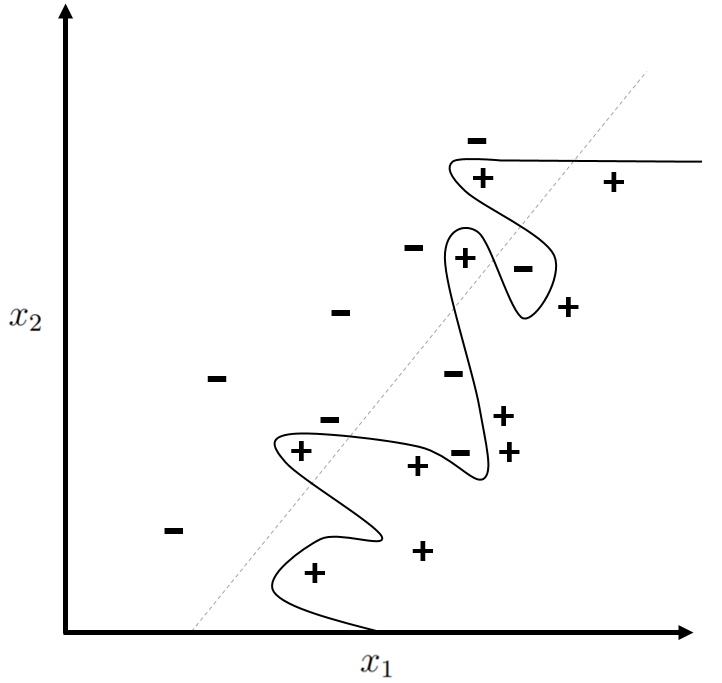
\includegraphics[scale=0.6]{figs/overfitting.png}
	\end{center}
	\caption{An example of the an overfitting function.}
	\label{fig:2dpoints}
\end{figure}
\section{Introduction to the Na\"{i}ve Bayes Classifier} \label{prep-bayes}

This is one of the simplest classifiers to understand and implement. It uses the assumption that all features are independent of each other:
\begin{equation}
	p(x_i | x_j) = p(x_i) \quad \forall i, j \in \mathbb{Z}^+.
\end{equation}
We say that the classifier is 'na\"{i}ve' because of this assumption. Although the assumption is very rarely true, the classifier still provides good performance \cite{ml_book_murphy}.
\newline
\newline
In addition to this assumption, the classifier uses Bayes Theorem:
\begin{equation}
	P(A | B) = \frac{P(B | A)P(A)}{P(B)}.
\end{equation}
The intuition behind the classifier is that given a set of features $\mathbf{x}$, we should assign it to the class that has the highest probability, given the set of features. Using the assumption of conditional independence and Bayes Theorem, we can compute this probability as follows:
\begin{equation}
\begin{aligned}
p(C = y | \mathbf{x}) &= \frac{p(\mathbf{x} | C = y)p(C = y)}{p(\mathbf{x})} \\
&= \frac{p(x_1, \ldots, x_k | C = y)p(C = y)}{p(\mathbf{x})} \\
&= \frac{p(x_1, \ldots, x_k, C = y)}{p(\mathbf{x})} \\
&= \frac{p(x_1 | x_2, \ldots, x_k, C = y)p(x_2, \ldots, x_k, C = y)}{p(\mathbf{x})} \\
& \vdots \\
&= \frac{p(x_1 | x_2, \ldots, x_k, C = y)p(x_2 | x_3 \ldots, x_k, C = y)\cdots p(x_k | C = y)}{p(\mathbf{x})} \\
&= \frac{p(x_1 | C = y)p(x_2 | C = y) \cdots p(x_k | C = y)}{p(\mathbf{x})} \\
&= \frac{\prod_{i = 1}^{k}p(x_i | C = y)}{p(\mathbf{x})}. \\
\end{aligned}
\end{equation}

Clearly, this shows that we can compute y using:

\begin{equation}
\begin{aligned}
y &= \underset{y}{\operatorname{argmax}}\bigg(\frac{\prod_{i = 1}^{k}p(x_i | C = y)}{p(\mathbf{x})}\bigg) \\
&= \underset{y}{\operatorname{argmax}} \displaystyle \prod_{i = 1}^{k}p(x_i | C = y). \\
\end{aligned}
\end{equation}

We can estimate each $p(x_i | C = y)$ trivially using the training data. Given that in this project I am only considering binary classifiers, where $y \in {-1, +1}$, we can write this as:

\begin{equation}
\text{max} \bigg( \displaystyle \prod_{i = 1}^{k}p(x_i | C = -1), \prod_{i = 1}^{k}p(x_i | C = +1) \bigg). \\
\end{equation}

Due to its simplicity and good performance, I will use the na\"{i}ve Bayes classifier as a baseline for my project.
\section{Introduction to Support Vector Machines} \label{prep-svm}

Support vector machines (SVMs) are widely used, state-of-the-art classifiers which were designed for binary classification (although they have since been modified to work for multi-class classification) \cite{ml_book}. Since I am viewing the task of determining the sentiment of speeches on the Iraq war as a binary classification problem, using a SVM is a natural choice.
\newline
\newline
In contrast to the na\"{i}ve Bayes classifier, the SVM approach to classification is not inherently probabilistic. Instead, they are a form of maximum margin classifier. A maximum margin classifier computes a hyperplane of the form
\begin{equation} \label{eq:hyperplane}
	\mathbf{w} \cdot \mathbf{x} + b = 0.
\end{equation}
where $\mathbf{w}$ is a normal to the hyperplane. $\mathbf{w}$ and $b$ are determined by the maximisation (\ref{eq:maxdelta}) and $\mathbf{x}$ is a point on the hyperplane. This hyperplane separates the training data, so that for all positive examples
\begin{equation}
\mathbf{w} \cdot \mathbf{x} + b \ge 0
\end{equation}
and for all negative examples
\begin{equation}
\mathbf{w} \cdot \mathbf{x} + b < 0.
\end{equation}
The idea of the maximum margin classifier is that it maximises $\delta$, the distance between the hyperplane and the closest examples to it. That is, it computes
\begin{equation} \label{eq:maxdelta}
	\underset{\mathbf{w}, b}{\operatorname{argmax}}(min(\delta)).
\end{equation}
Figure \ref{fig:hyperplane} illustrates this problem in a 2D space (i.e. where $\mathbf{x} = (x_1, x_2)$).
\begin{figure}
	\begin{center}
		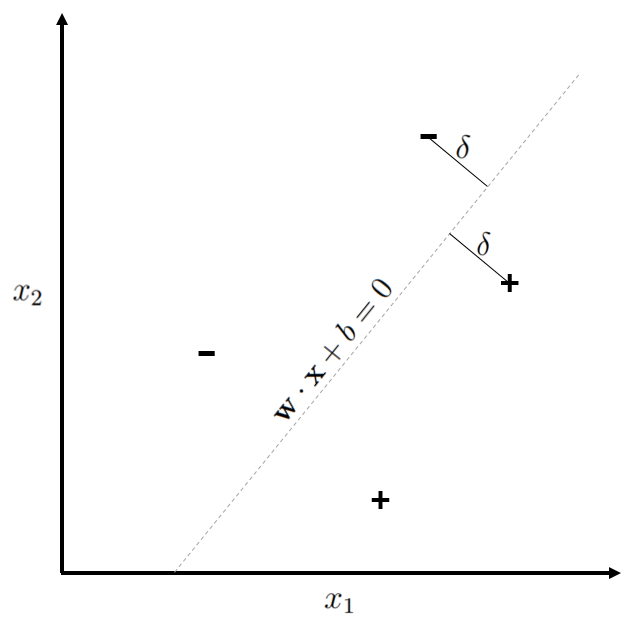
\includegraphics[scale=0.6]{figs/hyperplane.png}
	\end{center}
	\caption{A simple 2D plot of four labelled features and a hyperplane (which is a line in two dimensions) distinguishing the positive and negative points.}
	\label{fig:hyperplane}
\end{figure}
\newline
\newline
To determine whether feature vector $\mathbf{x}_i$ should be positively or negatively labelled, we simply need to determine which side of the hyperplane it lies on. This gives us the decision function
\begin{equation} \label{eq:initialdecision}
	y_i =
	\begin{cases}
		+1, \quad \mathbf{w} \cdot \mathbf{u} + b \ge 0 \\
		-1, \quad \text{otherwise}
	\end{cases}
\end{equation}
where $\mathbf{u}$ is the feature vector being classified. The support vectors are defined as the training examples that lie closest to the hyperplane. From the equation of the hyperplane (\ref{eq:hyperplane}), we see that we have the freedom to scale $\mathbf{w}$ and $b$ by a constant factor without changing the hyperplane itself. We can therefore define this scaling by imposing the following constraint on all training examples for mathematical convenience:
\begin{equation}
	y_i(\mathbf{w} \cdot \mathbf{x}_i + b) - 1 \ge 0.
\end{equation}
For the support vectors, we then have
\begin{align}
	& y_i(\mathbf{w} \cdot \mathbf{x}_i + b) - 1 = 0 \label{eq:svconstraint}\\
	\implies & \mathbf{w} \cdot \mathbf{x}_i = \frac{1}{y_i} - b. \label{eq:wdotx} \\
	\implies & b = \frac{1}{y_i} - \mathbf{w} \cdot \mathbf{x}_i. \label{eq:b}
\end{align}
%Insert figure
\newline
\newline
We now need to compute the width of the margin so we can then form an expression to maximise it. Figure \ref{fig:hyperplane} gives us some intuition as to how we can achieve this. Since $\mathbf{w}$ is perpendicular to the hyperplane, $\frac{\mathbf{w}}{||\mathbf{w}||}$ must be the unit normal to the hyperplane. We can then use a positively labelled support vector, $\mathbf{x}_+$ and a negatively labelled support vector, $\mathbf{x}_-$ to get an expression for the margin width:
\begin{equation}
\begin{aligned}
	\text{Margin width} & = \frac{\mathbf{w}}{||\mathbf{w}||} \cdot (\mathbf{x}_+ - \mathbf{x}_-) \\
	& = \frac{\mathbf{w} \cdot \mathbf{x}_+ - \mathbf{w} \cdot \mathbf{x}_-}{||\mathbf{w}||}
\end{aligned}
\end{equation}
We can now substitute in the result from (\ref{eq:wdotx}) to give
\begin{equation} \label{eq:width}
\begin{aligned}
\text{Margin width} & = \frac{\big(\frac{1}{y_+} - b\big) - \big(\frac{1}{y_-} - b\big)}{||\mathbf{w}||} \\
& = \frac{\frac{1}{y_+} - \frac{1}{y_-}}{||\mathbf{w}||} \\
& = \frac{1 + 1}{||\mathbf{w}||} \\
& = \frac{2}{||\mathbf{w}||} \\
\end{aligned}
\end{equation}
Our goal is to maximise the width given by (\ref{eq:width}). For mathematical convenience, we can instead solve the equivalent problem of minimising $\frac{1}{2}||\mathbf{w}||^2$. This optimisation is subject to the constraints in (\ref{eq:svconstraint}). In order to solve this constrained optimisation problem, we must use Lagrange multipliers
\begin{equation}
	\boldsymbol{\alpha} = (\alpha_1, \alpha_2, \ldots, \alpha_n)
\end{equation}
where $n$ is the number of training examples. This results in the Lagrange function
\begin{equation} \label{eq:initialL}
	L = \frac{1}{2}||\mathbf{w}||^2 - \sum_{i = 1}^{n} \alpha_i (y_i(\mathbf{w} \cdot \mathbf{x}_i + b) - 1). 
\end{equation}
Our task is now to solve the unconstrained maximisation problem
\begin{equation} \label{eq:lagrangeoptimisation}
	(\mathbf{w}_{opt}, b_{opt}) = \underset{\mathbf{w}, b}{\operatorname{argmax}}(L)
\end{equation}
Using the Karush-Kuhn-Tucker conditions, we can show that $\alpha_i = 0$ for all feature vectors that are not support vectors \cite{ml_book}. This results in fast computation and means that after training, we only need to store the support vectors. Therefore, from now on, we will sum over $\mathcal{S}$, the set of indices corresponding to the support vectors.
\newline
\newline
In order to solve the optimisation problem defined in (\ref{eq:lagrangeoptimisation}), we must find the partial derivative of L with respect to both $\mathbf{w}$ and $b$, setting the resulting expressions to 0 (since we want to vary $\mathbf{w}$ and $b$ in order to find the maximum L).
\begin{align}
	\frac{\partial L}{\partial \mathbf{w}} & = \mathbf{w} - \sum_{i \in \mathcal{S}} \alpha_i y_i \mathbf{x}_i = 0 \\
	\implies \mathbf{w} & = \sum_{i \in \mathcal{S}} \alpha_i y_i \mathbf{x}_i \label{eq:wsum} \\
	\frac{\partial L}{\partial b} & = \sum_{i \in \mathcal{S}} \alpha_i y_i = 0 \label{eq:db}
\end{align}
We can now substitute (\ref{eq:wsum}) into (\ref{eq:initialL}) to obtain a new expression for $L$ (and simplify using (\ref{eq:db})) as follows:
\begin{equation} \label{eq:separableL}
\begin{aligned}
	L & = \frac{1}{2}(\sum_{i \in \mathcal{S}} \alpha_i y_i \mathbf{x}_i)(\sum_{j \in \mathcal{S}} \alpha_j y_j \mathbf{x}_j) - \sum_{i \in \mathcal{S}} \alpha_i y_i(\sum_{j \in \mathcal{S}} \alpha_j y_j \mathbf{x}_j) \cdot \mathbf{x}_i - b\sum_{i \in \mathcal{S}} \alpha_i y_i + \sum_{i \in \mathcal{S}} \alpha_i \\
	& = \frac{1}{2}(\sum_{i \in \mathcal{S}} \alpha_i y_i \mathbf{x}_i)(\sum_{j \in \mathcal{S}} \alpha_j y_j \mathbf{x}_j) - (\sum_{i \in \mathcal{S}} \alpha_i y_i \mathbf{x}_i)(\sum_{j \in \mathcal{S}} \alpha_j y_j \mathbf{x}_j) + \sum_{i \in \mathcal{S}} \alpha_i \\
	& = \sum_{i \in \mathcal{S}} \alpha_i - \frac{1}{2}(\sum_{i \in \mathcal{S}} \alpha_i y_i \mathbf{x}_i)(\sum_{j \in \mathcal{S}} \alpha_j y_j \mathbf{x}_j) \\
	& = \sum_{i \in \mathcal{S}} \alpha_i - \frac{1}{2}\sum_{i \in \mathcal{S}} \sum_{j \in \mathcal{S}} \alpha_i \alpha_j y_i y_j (\mathbf{x}_i \cdot \mathbf{x}_j). \\
\end{aligned}
\end{equation}
We now need to find the values $\boldsymbol{\alpha}$ which maximise L:
\begin{equation} \label{eq:maximisation}
	\boldsymbol{\alpha}_{opt} = \underset{\boldsymbol{\alpha}}{\operatorname{argmax}}(L).
\end{equation}
I won't go into the details of how to find these values, but this can be done numerically. Further to this, it can be shown that the space of $L$ is convex, so we will not find a local maximum. This is a significant advantage of using SVMs over neural networks.
\newline
\newline
We can then find $\mathbf{w}_{opt}$ by substituting $\boldsymbol{\alpha}_{opt}$ into (\ref{eq:wsum}) and using the support vectors and their labels. From this, we can find $b_{opt}$ using (\ref{eq:b}) and substituting in $\mathbf{w}_{opt}$ along with any support vector and its label. We can substitute our values for $\boldsymbol{\alpha}_{opt}$ and $b_{opt}$ into the initial decision rule to obtain a new decision rule:
\begin{equation} \label{eq:separabledecision}
	y_i =
	\begin{cases}
		+1, \quad \displaystyle \sum_{i \in \mathcal{S}} y_i(\boldsymbol{\alpha}_{opt})_i (\mathbf{x}_i \cdot \mathbf{u}) + b \ge 0 \\
		-1, \quad \text{otherwise}.
	\end{cases}
\end{equation}
Thus far, we have been working under the assumption that our data is linearly separable. In practice, this is very rarely the case and for this project due to the inherent noise in our data (described in \S \ref{intro-challenges}), this assumption is very unlikely to hold. Figure \ref{fig:inseparable} illustrates a simple example for which the data are not linearly separable.
\begin{figure}
	\begin{center}
		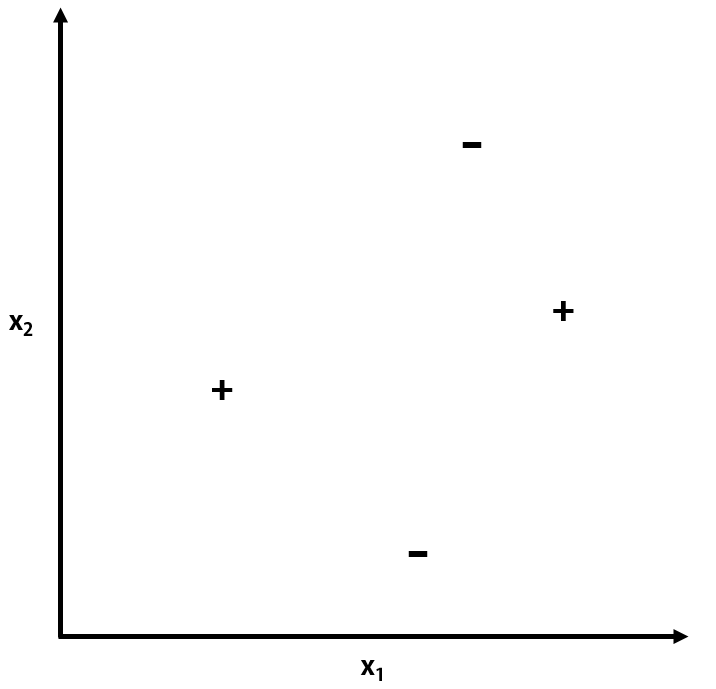
\includegraphics[scale=0.6]{figs/inseparable.png}
	\end{center}
	\caption{A simple 2D plot of four linearly inseparable labelled features.}
	\label{fig:inseparable}
\end{figure}
\newline
\newline
In order to fix this problem, we can use a transformation, $\phi$, to transform our feature vectors into a new space in which our data is more easily separable. Applying this transformation to (\ref{eq:separableL}) gives us a new $L$:
\begin{equation} \label{eq:phiL}
	L = \sum_{i \in \mathcal{S}} \alpha_i - \frac{1}{2}\sum_{i \in \mathcal{S}} \sum_{j \in \mathcal{S}} \alpha_i \alpha_j y_i y_j (\phi (\mathbf{x}_i) \cdot \phi (\mathbf{x}_j)).
\end{equation}
We maximise this as before, finding a new $\boldsymbol{\alpha}_{opt}$ from (\ref{eq:maximisation}) and then using those values to find $b_{opt}$. We can then use these values of $\boldsymbol{\alpha}_{opt}$ and $b_{opt}$ along with the transformation $\phi$ to obtain another decision rule:
\begin{equation} \label{eq:phidecision}
	y_i =
	\begin{cases}
		+1, \quad \displaystyle \sum_{i \in \mathcal{S}} y_i(\boldsymbol{\alpha}_{opt})_i (\phi (\mathbf{x}_i) \cdot \phi (\mathbf{u})) + b \ge 0 \\
		-1, \quad \text{otherwise}.
	\end{cases}
\end{equation}
We are yet to define $\phi$, but if we consider the contexts in which it is used, we see that it is always in the form $\phi (\mathbf{x}) \cdot \phi (\mathbf{x}')$. Therefore, rather than define $\phi$ itself, we define a kernel function
\begin{equation}
	k(\mathbf{x}, \mathbf{x}') = \phi (\mathbf{x}) \cdot \phi (\mathbf{x}').
\end{equation}
From this, we can rewrite (\ref{eq:phiL}) and (\ref{eq:phidecision}) as:
\begin{equation}
	L = \sum_{i \in \mathcal{S}} \alpha_i - \frac{1}{2}\sum_{i \in \mathcal{S}} \sum_{j \in \mathcal{S}} \alpha_i \alpha_j y_i y_j k(\mathbf{x}_i, \mathbf{x}_j) \\
\end{equation}
\begin{equation}
	y_i =
	\begin{cases}
		+1, \quad \displaystyle \sum_{i \in \mathcal{S}} y_i(\boldsymbol{\alpha}_{opt})_i k(\mathbf{x}_i, \mathbf{u}) + b \ge 0 \\
		-1, \quad \text{otherwise}.
	\end{cases}
\end{equation}
The choice of kernel function can have a significant effect on the performance of a SVM. In order to ensure good results, I will train the SVM using different kernel functions, so the classifier learns which kernel function will work best for the data. The three kernel functions I will consider are:
\begin{align}
	k(\mathbf{x}, \mathbf{x}') & = \mathbf{x} \cdot \mathbf{x}'& \label{eq:linearkernel} \\
	k(\mathbf{x}, \mathbf{x}') & = (\gamma (\mathbf{x} \cdot \mathbf{x}') + r)^d \quad & \gamma \in \mathbb{R}_{> 0} . r \in \mathbb{R}_{\ge 0} . d \in \mathbb{N}_{> 0} \label{eq:polykernel} \\
	k(\mathbf{x}, \mathbf{x}') & = e^{-\gamma ||\mathbf{x} - \mathbf{x}'||^2} \quad & \gamma \in \mathbb{R}_{> 0} \label{eq:rbfkernel}
\end{align}
From now on, I will refer to (\ref{eq:linearkernel}), (\ref{eq:polykernel}) and (\ref{eq:rbfkernel}) as the linear kernel, the polynomial kernel and the radial basis function (rbf) kernel respectively. Using the linear kernel is equivalent to our SVM before we introduced the transformation $\phi$. This shows that even with kernel functions, our data may not be linearly separable. It can be shown that linear and polynomial kernels do not necessarily transform the data so that into a space in which it is linearly separable, but the rbf kernel can always map the feature vectors to a space where they are linearly separable. This means that for the linear and polynomial kernels, we may not be able to produce a classifier with the given constraints and for the rbf kernel the SVM is very susceptible to overfitting. Both of these problems can be solved by introducing soft-margins to our SVM. This means that we will allow the SVM to incorrectly classify some of the training examples. In order to do this, we introduce a parameter $C$ which trades off correct classification of training examples with a greater margin width. A greater margin width results in a smoother function, so means that the SVM is less likely to overfit. The higher the value of $C$, the more training examples the SVM will fit correctly. $C$ is a hyperparameter - that is a parameter whose value is fixed before the classifier is trained. All of the hyperparameters for each of the kernels we are considering are shown in Table \ref{table:hyperparameters}. The hyperparameter choice significantly effects the performance of the SVM, so we need an algorithm for choosing them. This is discussed further in both \S\ref{cross-validation} \& \S\ref{impl-classifier}.
\FloatBarrier
\begin{table}[]
	\centering
	\label{table:hyperparameters}
	\begin{tabular}{ll}
		\textbf{Kernel}       & \textbf{Hyperparameters} \\ \hline
		Linear                & $C$                      \\
		Polynomial            & $C$, $\gamma$, $r$, $d$  \\
		Radial basis function & $C$, $\gamma$             
	\end{tabular}
	\caption{The hyperparameters of various kernels}
\end{table}
\FloatBarrier
\section{Introduction to Evaluating Supervised Learning Systems} \label{prep-eval}
\subsection{Train/Test Split} \label{train-test-split}
In \S\ref{supervised-learning}, we saw how a supervised learning system is trained on one set of data (the training set), then this trained model is used to predict the labels of previously unseen data (the testing set). In order to evaluate a system, we require the actual data labels, so we can assess the accuracy of the predictions. Having training examples in the testing set results will not provide a useful measure of the system's performance, as it would unfairly reward overfitting. In order to overcome this, we must split our labelled data before we start developing a model. Using 90\% for training and 10\% for testing is the most common way to split the labelled data.
\subsection{Overfitting} \label{prep-overfitting}

Overfitting is a common problem in supervised learning problems. It occurs when a classifier learns to get a very high performance on the training set, but does not generalise well to unseen data, meaning that the classifier achieves poor results on the test data. Figure \ref{fig:overfitting} illustrates a simple example of a (two-dimensional) hyperplane overfits the given data.

\subsection{Cross Validation} \label{cross-validation}
Cross validation is a way to mitigate overfitting. To use this scheme, we split the training set into $k$ disjoint folds. Doing this means that we can iterate the process of training and evaluating without using the data set aside for testing. This is done by training on $k-1$ of the folds, then evaluating the system on the fold left out. This is repeated $k$ times, so each fold is used for evaluation exactly once. Averaging over all the folds each fold gives a reliable evaluation metric. We can use this method to determine the system's hyperparameters and any other settings that need to be determined before training. This is called cross-validation. To do this, we repeat the method described for different combinations of hyperparameters and settings and select the combination whose average evaluation metric is greatest. In this project, I use stratified cross-validation - for this scheme, when splitting the data into folds, I ensure that each fold has a roughly even split of positive and negative examples.
\subsection{Evaluation Metrics} \label{evaluation-metrics}
Thus far, we have only spoken abstractly about an evaluation metric. There are various options and choice of the measure should be context-specific. The basis of the definitions used in most metrics are defined in the Table \ref{table:true-positives}.
\FloatBarrier
\begin{table}[]
	\centering
	\label{table:true-positives}
	\begin{tabular}{llll}
		&                                                                    & \multicolumn{2}{c}{Prediction} \\
		& \multicolumn{1}{l|}{}                                              & \textbf{Positive}  & \textbf{Negative}  \\ \cline{2-4} 
		\multirow{2}{*}{Actual Value}&\multicolumn{1}{l|}{\textbf{Positive}} & True Positive      & False Negative     \\
		& \multicolumn{1}{l|}{\textbf{Negative}}                             & False Positive     & True Negative     
	\end{tabular}
	\caption{Defining true positives, true negatives, false positives and false negatives}
\end{table}
\FloatBarrier
From this, we can now define the following quantities:
\begin{align}
	TP & = \text{Number of True Positives} \\
	FN & = \text{Number of False Negatives} \\
	FP & = \text{Number of False Positives} \\
	TN & = \text{Number of True Negatives}
\end{align}
Accuracy is the simplest evaluation metric. We define this as:
\begin{equation}
	\text{Accuracy} = \frac{TP + TN}{TP + FN + FP + TN}
\end{equation}
If we have an unbalanced dataset (which is the case in this project), then accuracy is not a good evaluation metric. To illustrate this, consider the case where 1\% of our data is positive and 99\% of our data is negative. If we had a classifier that always predicted that an example was negative, its accuracy would be 99\%. Since accuracy is not a useful measure for unbalanced datasets, such as the dataset I am using in this project, I will not consider it any further.
\newline
\newline
We now define two further measures:
\begin{align}
	\text{Precision} & = \frac{TP}{TP + FP} \\
	\text{Recall} & = \frac{TP}{TP + FN}
\end{align}
A good evaluation metric for an unbalanced dataset will incorporate some trade-off between precision and recall. Such a metric may give greater weighting to precision for a precision-critical task or greater weighting to recall for a recall-critical task. Since this project is neither precision-critical nor recall-critical, we can use the $F_1$ score as the evaluation metric, since the $F_1$ score is defined as the harmonic mean of precision and recall:
\begin{equation}
	F_1 = \frac{2 \times \text{precision} \times \text{recall}}{\text{precision} + \text{recall}}.
\end{equation}
\section{Introduction to the Bag-of-Words Model} \label{prep-bow}

In mathematics, a bag is a synonym for a multiset - an abstract data type which is like a set, but differs in that it can contain duplicates. In this project, I will represent MPs' speeches using a bag-of-words model, meaning that the representation ignores the order of words. Despite its simplicity, the bag-of-words model is used successfully in a range of sentiment classification applications, as it can effectively capture the discourse of a text \cite{nlp_book}.
\newline
\newline
To illustrate a bag-of-words model using an example, I will use an quote from a House of Commons debate on 18th March 2003:
\begin{center}
	\textit{``The best way to avoid war is to work through the United Nations.''}
	\newline
	 - Bill Tynan (Labour Party)
\end{center}
In a simple bag-of-words implementation, where case and punctuation are ignored, this sentence would be stored as:
\begin{align*}
	\{\text{the}&: 2,\\ \text{to}&: 2,\\ \text{best}&: 1,\\ \text{way}&: 1,\\ \text{avoid}&: 1,\\ \text{war}&: 1,\\ \text{is}&: 1,\\ \text{work}&: 1,\\ \text{through}&: 1,\\ \text{united}&: 1,\\ \text{nations}&: 1\}.
\end{align*}
It is important to note that the order of the elements above is not relevant.

\section{Software Engineering Techniques} \label{prep-sweng}
	
Before implementing the first classifier, I couldn't be sure that it would be possible to develop a system to classify MP's speeches due to the lack of other similar work. Due to this, it was important to get to this point as quickly as possible and then change the project requirements at that point if the data couldn't be classified. This strategy lent itself to agile software development \cite{agile}, so this is what I used. I used each of the tasks in Table \ref{table:tasks} to establish the projects first sprints, later defining further sprints as project extensions.
\newline
\newline
Throughout development, I used a linter to ensure that I maintained a high standard of code, with consistent documentation and also used revision control. I designed programs to be as modular as possible, which helped with testing and debugging.
\newline
\newline
Development of machine learning systems requires further good practices to be adopted, to avoid overfitting. To this end, as soon as I had constructed the database, I split the data into a training set and a testing set. Throughout the implementation, I solely used the training set, carrying out cross-validation across it to test code then using the testing set for evaluation. Further to this, before classifying MPs' speeches, I implemented a classifier for spam emails (see \S\ref{eval-spam}) and then adapted this classifier for the purposes of this project.


\section{Choice of Tools} \label{prep-tools}

\subsection{Programming Language}

I decided to develop the project in Python for various reasons:
\begin{itemize}
	\item There are many good natural language processing and supervised learning libraries available for Python.
	\item Python is well-suited to agile development.
	\item Python has a lot of community support available.
	\item I have previously used Python for large software projects (working in industry).
\end{itemize}
I used Python 3.6 since it was the most recent stable version of Python when I started implementation.

\subsection{Database} \label{prep-database}

Due to the structure of the data, it made sense to use a relational database. After considering various options, I opted to use SQLite due to its low set-up overheads (which is useful for agile development), its stability and its compatibility with Python.

\subsection{Libraries} \label{prep-tools-libs}

I used BeautifulSoup to parse the Hansard's html and the .ems files from the spam email dataset. Although lxml is a faster parser \cite{parsing}, BeautifulSoup copes better with `broken' html. Before implementation, I found various inconsistencies with the Hansard's html so BeautifulSoup was a better choice (especially since there were no significant time constraints on parsing). The Natural Language Toolkit is a widely used library with multiple functions, so I used this for various things. Similarly, I used functions from scikit-learn when implementing the classifier. In order to perform fast mathematical computations I used both NumPy and SciPy. In order to perform fast HTTP requests, I used the Requests library. In addition to the libraries mentioned, I also used different modules from the Python standard library.

\subsection{Development Environment}

I predominantly developed the project using my own laptop running the Windows 10 operating system. I used Visual Studio Code as the source code editor, with Python and PyLint extensions. One advantage of using Visual Studio Code is the easy integration with git, which I used for revision control of both the Python source code and this dissertation's \LaTeX \space source code. Since I used git for revision control, I used GitHub to backup the source code. I also synced all of my dissertation files to Google Drive and periodically backed them up to an external disk.

\subsection{Table of Software Used}
\begin{table}[H]
	\centering
	\label{table:software}
	\begin{tabular}{ll}
		\textbf{Software}        & \textbf{Version} \\ \hline
		BeautifulSoup            & 4.6.0            \\
		git                      & 2.8.1.windows.1  \\
		Natural Language Toolkit & 3.2.5            \\
		NumPy                    & 1.13.3           \\
		PyLint                   & 1.7.4            \\
		Python                   & 3.6.3            \\
		Requests                 & 2.18.4           \\
		Scikit-Learn             & 0.0              \\
		SciPy                    & 1.0.0            \\
		SQLite                   & 3.10.1           \\
		Visual Studio Code       & 1.20.1           \\
		Windows 10               & Home             \\
	\end{tabular}
	\caption{The versions of the software used in this project}
\end{table}

\section{Summary}

In this chapter, I have defined the project and the steps I took before starting its development. These steps involved planning the project and how its success will be measured, thereby allowing smoother implementation and evaluation.

\chapter{Implementation} \label{impl}

This chapter discusses the implementation of the various components of the project. Section \S\ref{impl-architecture} provides an overview to the system's implementation. Section \S\ref{impl-structures} talks about some of the design decisions related to specific data structures. Section \S\ref{impl-acquisition} gives details about compiling the project's dataset and section \S\ref{impl-classifier} discusses the implementation of the classifier.


\section{System Architecture} \label{impl-architecture}

Through the requirements analysis in the preparation section (\S\ref{prep-requirements}), I established the project's core tasks and their dependences (see Table \ref{table:tasks}). From this, I was able to simply create a project timetable, broken down into sprints. Each of the project's core tasks was the milestone reached by a sprint. After completing the essential components of the project, I improved the classifier by implementing a series of extensions. The list below gives each of the sprints I carried out (including the extensions):

\begin{enumerate}
	\item Scrape the relevant data from the Hansard.
	\item Wrangle the textual data so it is in a more consistent form.
	\item Collate the data from the transcript with voting record data.
	\item Construct a database of the new dataset I have created.
	\item Parse the spam email dataset.
	\item Develop an SVM classifier to detect spam email.
	\item Develop a na\"{i}ve Bayes classifier to predict the stance of MPs' speeches.
	\item Use the spam email classifier as a basis to develop an SVM classifier to predict the stance of MPs' speeches on the Iraq war.
	\item Extension: Implement stop word removal, stemming, n-grams and number grouping.
	\item Extension: Implement an algorithm to allow the SVM classifiers to learn the best combination of settings and hyperparameters.
	\item Extension: Optimise the SVM classifiers by carrying out singular value decomposition on the feature vectors.
\end{enumerate}

As this project is very data intensive, I defined how data would flow before commencing implementation. Figure \ref{fig:dataflow} shows the movement of data between modules and data sources (including local files). Data moves in the direction of the arrows. This diagram shows the project's dependency on the Hansard, data.parliament.uk and the spam email dataset. I therefore ensured that I had a backed-up copies of the data from these sources at the earliest possible stage in the project, to mitigate any issues if the servers hosting these datasets went down at any point throughout the project.
\newline
\begin{figure}
	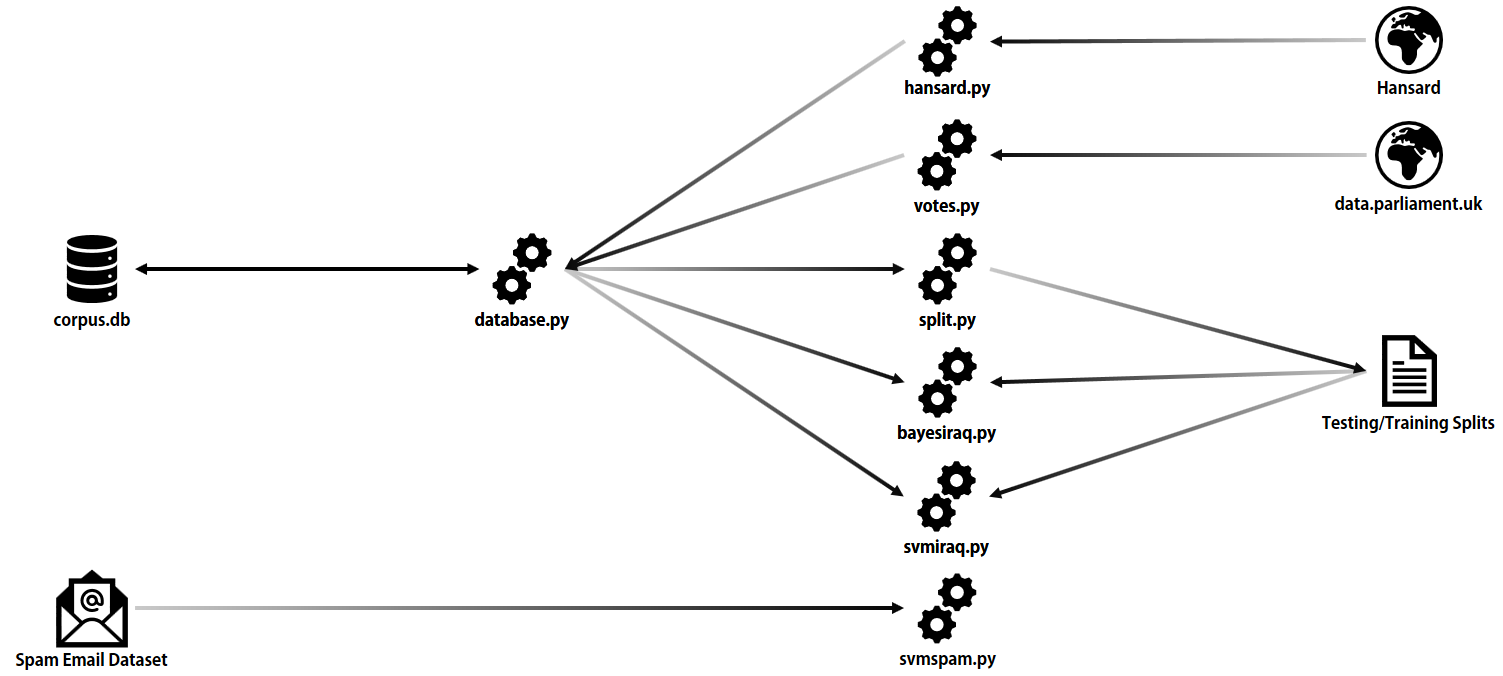
\includegraphics[width=\linewidth]{figs/dataflow3.png}
	\caption{Data flow in the project.}
	\label{fig:dataflow}
\end{figure}

Deciding upon this data flow, then allowed me to develop a finer project structure. Figure \ref{fig:dependencies} shows the internal dependencies of the modules in the project. An arrow from A to B indicates that A is dependent on B. Note that I designed the system in a way that avoids any cyclic dependencies and maximises code-sharing between modules.

\begin{figure}
	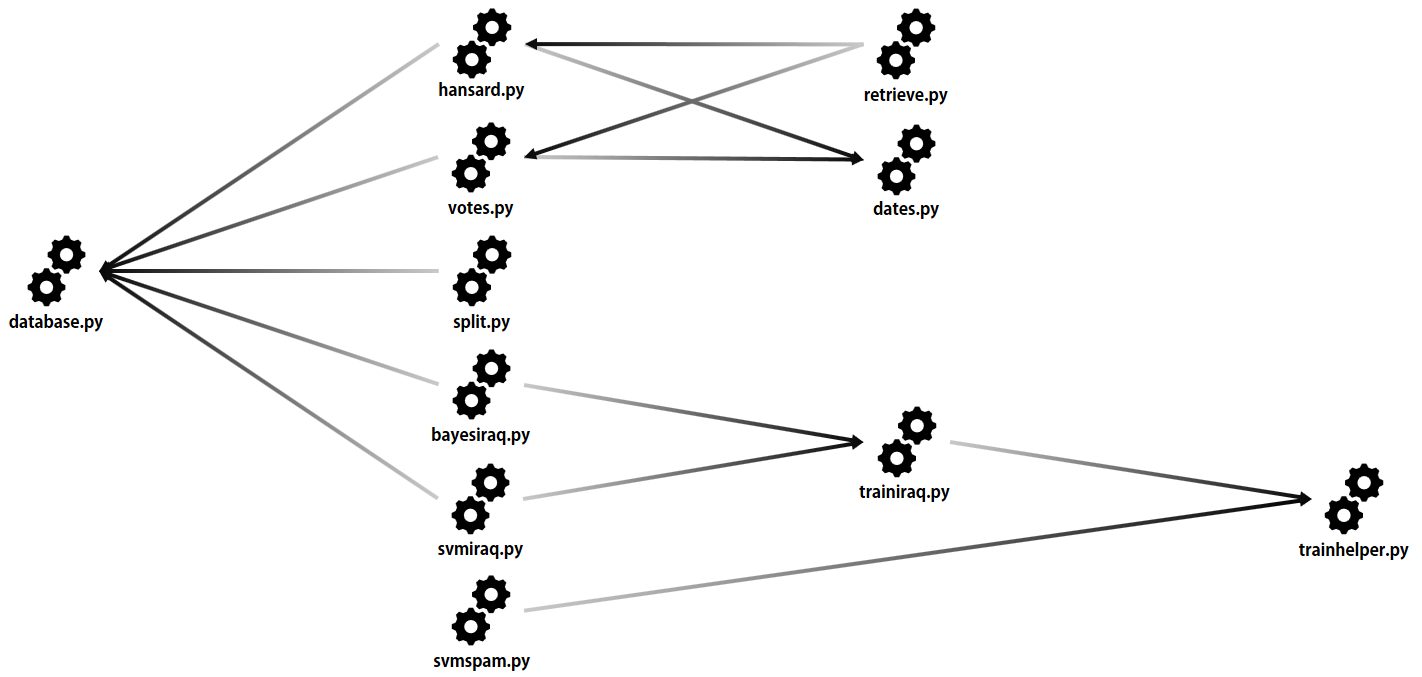
\includegraphics[width=\linewidth]{figs/internaldependencies.png}
	\caption{Internal dependencies within the project.}
	\label{fig:dependencies}
\end{figure}

\section{Data Structures} \label{impl-structures}

The size of the project means that I used a large variety of different data structures. In this section, I discuss the choice and use of a few of these data structures.

\subsection{NumPy Arrays}

I used various parts of the NumPy library throughout the project. For example, I frequently used NumPy arrays in situations where a simple Python list would have sufficed. For this project, NumPy arrays had various advantages over Python lists:
\begin{itemize}
	\item Operations on them are faster - they were specifically designed to with performance in mind, which Python was not \cite{numpyspeed}.
	\item They are more space efficient - their low-level implementation means that they use contiguous blocks of memory, rather than a series of pointers \cite{numpymanual}.
	\item They support matrix operations with no additional work.
\end{itemize}

The benefits of the first two points were particularly clear given the large amount of data I was processing. Since the features were the largest data structures I used for numerical computations, they made the advantages of using NumPy arrays clearest. Listing \ref{lst:reduce_features} gives a snippet of code which demonstrates my use of NumPy arrays.

\subsection{Sets}

The set data structure is built-in to Python and is implemented using a hash table \cite{pythonsetdocs}, meaning that lookup operations are performed in constant time. This in turn speeds up the implementation of other set functions, such as union, particularly for data which significantly overlap. For this reason, I used the Python set data type wherever it would improve the efficiency of a function.

\subsection{Counters} 

The Counter class is part of the collections module, which is part of the Python standard library, meaning that there is ample support available for its use. The data structure is optimised for counting hashable objects \cite{pythoncollectionsdocs}, meaning that it is essentially a multi-set designed to count the number of each element, which makes it perfect for representing a bag of words, making it useful throughout this project. As discussed in section \S\ref{impl-reduction}, it was necessary to reduce the size of the features used for classification, which could easily be done in $\mathcal{O}(k)$ time (where $k$ is the number of dimensions on the reduced features) using Counter's most\_common() method.

\section{Data Acquisition} \label{impl-acquisition}
\subsection{Scraping Data} \label{impl-scraping}

This section discusses how I got acquired the relevant data. The difficulty of this sprint of the project was that the transcript data that I required was not available in an API, so I had to scrape the data from the Hansard's inconsistently (and often incorrectly) structured web pages. This meant that I had to develop defensive code that handled lots of corner cases. As discussed in \S\ref{prep-tools-libs}, I opted to use BeautifulSoup to parse the .html files.
\newline
I developed a program that could traverse the Hansard to find the pages containing relevant debates. In order to do this, I iterated over all dates in the range I was considering\footnote{11/09/2001 to 18/03/2003 (inclusive)} and on each of these days, parsed the Hansard's webpage for that day and used this to find links to any relevant debates on that day. Figure \ref{fig:incorrecthansard} is one of many examples of incorrectly structured data in the Hansard - it suggests that all the debates on that day were prayers. Due to the Hansard's deficiencies, I had to exhaustively search through each House of Commons sitting, which significantly increased the running time of this part of the program. Listing \ref{lst:add_day} gives the high level code used to traverse the Hansard archives. The Hansard's inconsistencies required me to program defensively, by using extensive exception-handling.
\newline

\begin{figure}
	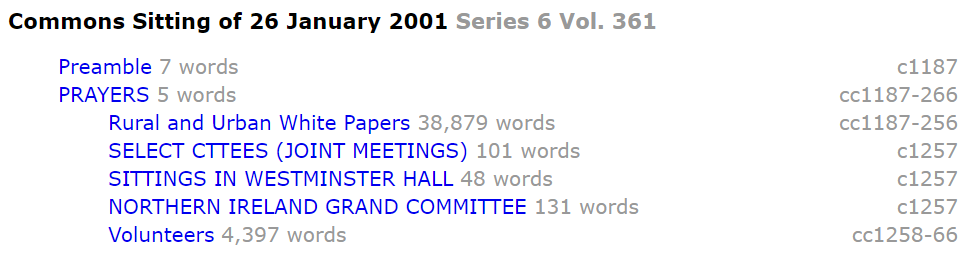
\includegraphics[width=\linewidth]{figs/incorrecthansard.png}
	\caption{A screenshot of incorrect structure in the Hansard.}
	\label{fig:incorrecthansard}
\end{figure}

\pylisting{High-level code used to scrape all the debates from a given day.}{add_day}

\subsection{Wrangling Data} \label{impl-wrangling}
When parsing the debates and quotes, I faced similar difficulties to parsing the Hansard's pages for each day, meaning that I again had to extensively use exception-handling. To illustrate some of the difficulties of using the Hansard to generate text that is suitable for classification, I have given provided Figure \ref{fig:hansardquote} which is a screenshot of a quote in the Hansard, along with Listing \ref{lst:quote}, which is the corresponding HTML paragraph tag. I have trimmed the HTML slightly, so it is easier to read. After reading through the HTML for a representative sample of debates in the Hansard, I wrote some functions to extract the relevant text from the Hansard's HTML, including the method given in Listing \ref{lst:quote}, which uses a series of regular expressions to make textual replacements.

\begin{figure}
	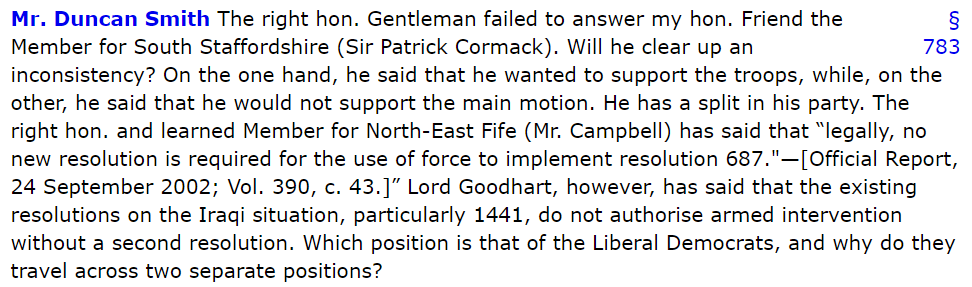
\includegraphics[width=\linewidth]{figs/idsquote.png}
	\caption{A screenshot of a quote in the Hansard.}
	\label{fig:hansardquote}
\end{figure}

\htmllisting{HTML paragraph tag of the quote in Figure \ref{fig:hansardquote}.}{quote}

\pylisting{Python code using regular expressions to clean the text from a paragraph tag.}{get_paragraph_text}
\subsection{Labelling Data} \label{impl-labelling}

One of my primary reasons for using the Hansard as the corpus for this project was the fact that I could label the data automatically, using MPs' voting records. This in turn meant that the project could be use supervised learning rather than unsupervised learning or semi-supervised learning. It was relatively trivial to retrieve voting data - I used the House of Commons Divisions API from data.parliament.uk.
\\\\
The main difficulty in labelling the data was matching the voting data with the transcript data. This issue was due to the fact that MPs' names varied greatly over time. For example, some MPs adopted married names during their time as an MP and some had titles that were intermittently used to refer to them. Michael Kerr is a good illustration of the multitude of names used by an individual - he is referred to as 13th Marquess of Lothian in the House of Commons Divisions API, the Earl of Ancram in the Hansard and is also known as Baron Kerr of Monteviot. Michael Kerr was one of 36 MPs whose name differed significantly enough between the two data sets that I couldn't algorithmically match their speeches with their voting record. These MPs were mostly unmatchable, due to maiden names, but I manually entered rules to handle them. I matched the other 619 MPs using the function given in Listing \ref{lst:match_full_name}. This method tries to match the given speaker with one of the MPs in the data.parliament.uk dataset, by removing any honorary titles from the speaker's name (since the data.parliament.uk dataset doesn't give these titles), then finding the most similar \footnote{Similarity is calculated using the Levenshtein distance, which is defined as the distance is the number of deletions, insertions, or substitutions required to convert one string into another.} name in the voting record dataset. If this name is deemed to be sufficiently similar, the speaker is matched. If it isn't, a similar function is called, which uses different data in the data.parliament.uk dataset to match the speaker. If this function cannot find a good match either, it raises a `MatchException', which is unhandled by the code in Listing \ref{lst:match_full_name}, meaning that match\_full\_name() also raises this exception. The code that handles these exceptions created a file of any unmatched MPs, which I subsequently manually looked up to find alternative names for the MPs. In order to minimise run-time, I kept a match list, so that once a match was found for a given MP, the same match could be found in constant time, since I used a Python dictionary (which is implemented using a hash table \cite{pythonfaqs}).

\pylisting{Function that matches an MP's name in the Hansard }{match_full_name}

\subsection{Database} \label{impl-database}

Since the database would only be used locally (so there would only ever be one copy) and I planned on accessing it serially, I could easily ensure that my database would satisfy the ACID properties (Atomicity, Consistency, Isolation \& Durability) by using a relational database. As described in \S\ref{prep-database}, I opted to use SQLite due to its low overheads - it is referred to as a zero-configuration database \cite{sqlitezeroconfig}. The benefits of this are two-fold; it reduces development time and running time, since there is no separate server process and therefore no overhead from message passing to and from the database \cite{sqliteserverless}. Further to this, the authors of SQLite released the code under a licence that allows anyone to ``copy, modify, publish, use, compile, sell, or distribute'' SQLite \cite{sqlitelicence}, which is clearly sufficient for my needs in this project.
\\\\
When designing the database schema, I ensured that the database would be fully normalised (in third normal form), which meant that the data would preserve referential integrity and minimise the potential for data duplication. Figure \ref{fig:erdiagram} shows the entity-relationship diagram for the database schema I adopted. Note that due to the limited type system in SQLite \cite{sqlitetypes}, all fields are of type `TEXT'. This is not a problem, because SQLite has built-in functions to handle data as if they were of different types - for example, the DEBATE and DIVISION entities had DATE attributes, which were represented as text in the database file, I could handle them easily as if they were of a type `DATE'.
\\\\
\begin{figure}
	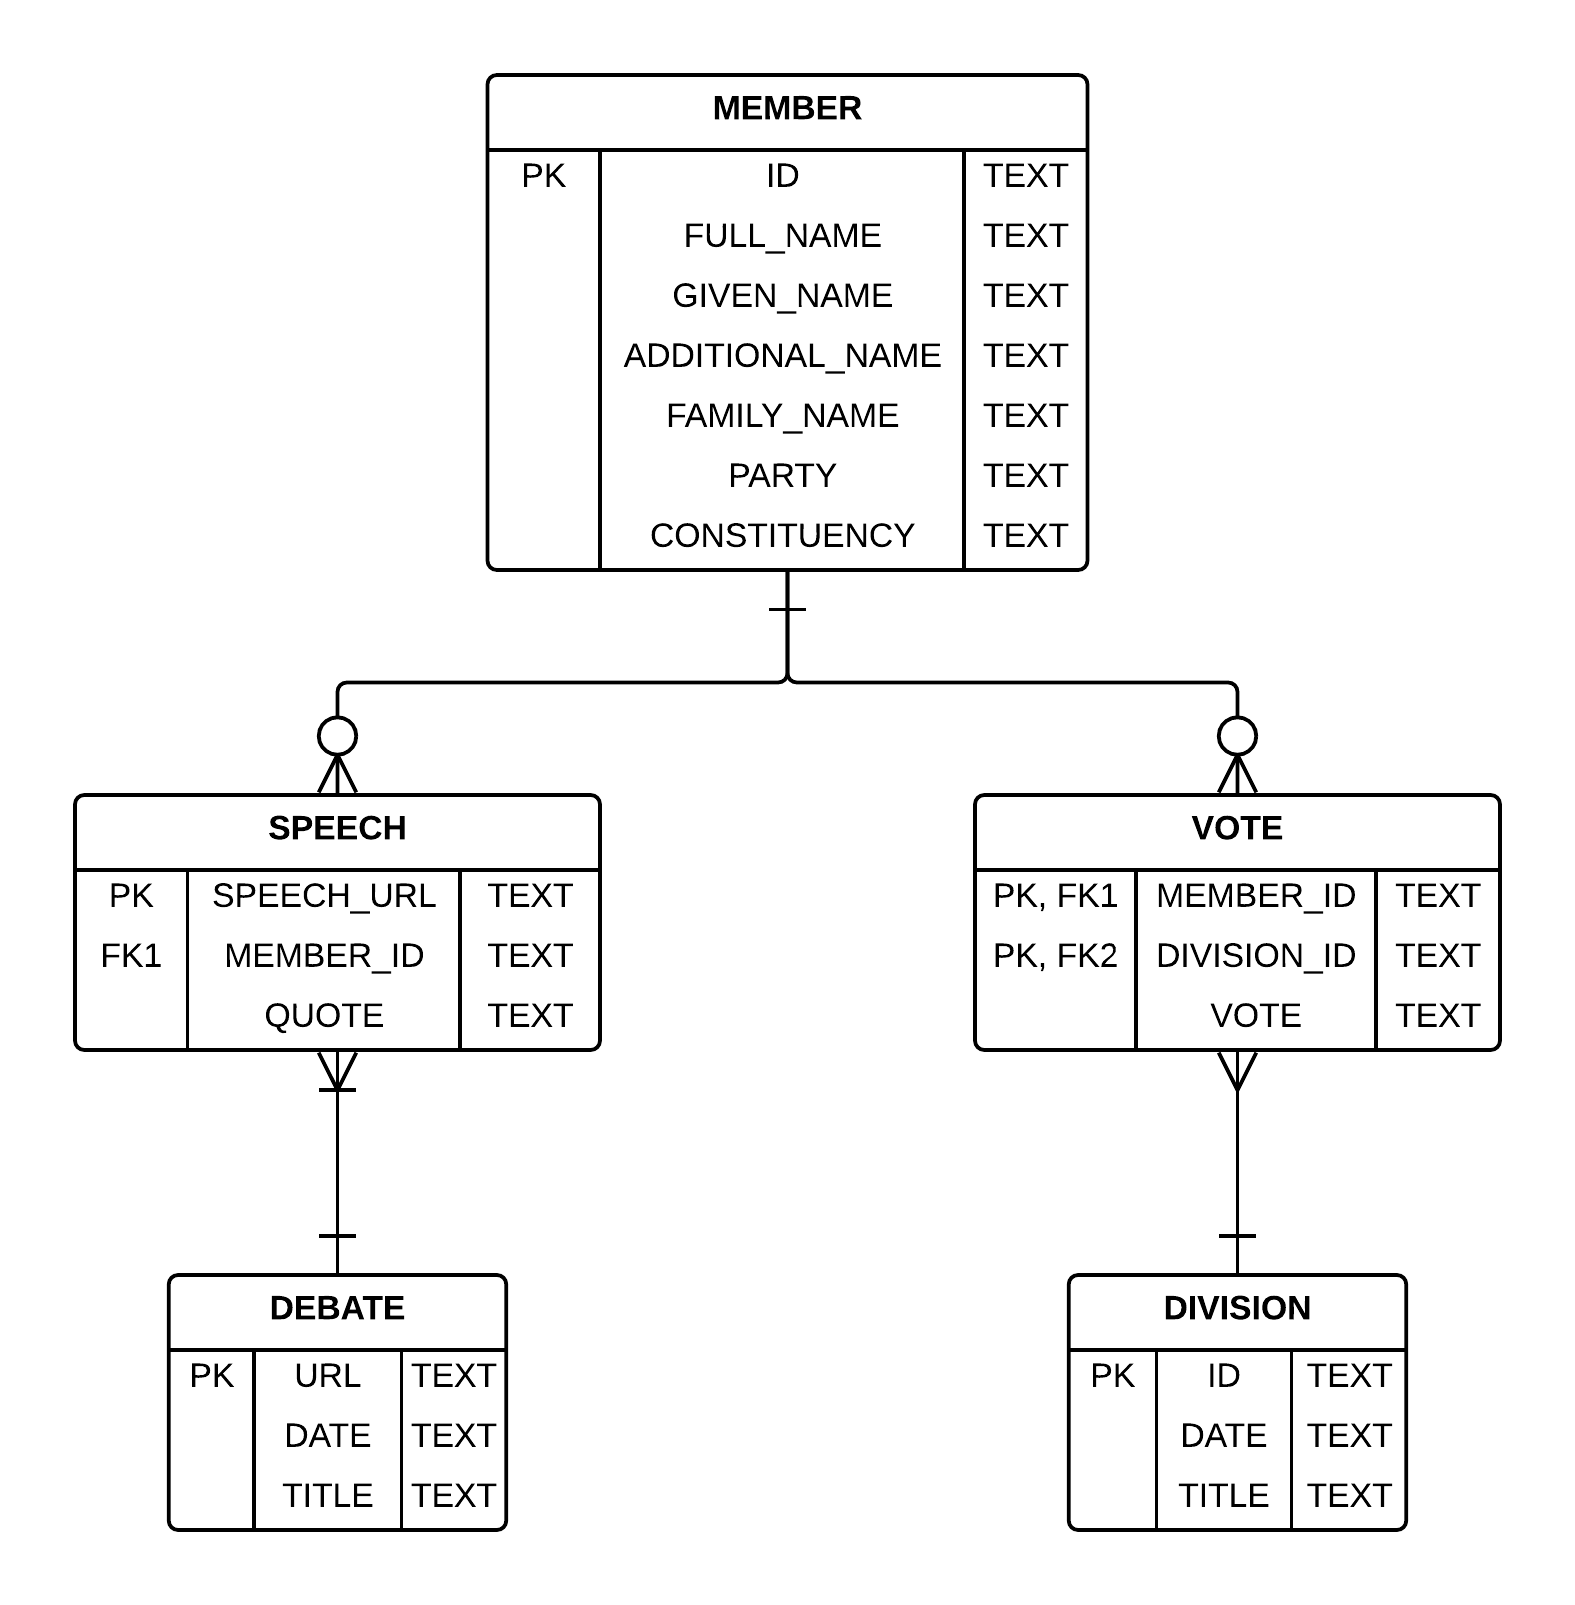
\includegraphics[width=\linewidth]{figs/erd.png}
	\caption{The entity-relationship (ER) diagram of the system's database.}
	\label{fig:erdiagram}
\end{figure}
When working with the database, it was useful to be able to manually check the data and therefore the functioning of any program using the database. To do this, I used DB Browser for SQLite, which is a lightweight GUI interface that allowed me to browse the data. This was particularly useful for `evaluating' the data acquisition, since there is no formal way for me to automatically check the data in the database. This meant that manually sampling the data using DB Browser for SQLite and cross-referencing the data with that in the original data sources was the best feasible way for me to evaluate the data acquisition.
\\\\
To maintain good software engineering practices, I only accessed the database through the database class (as shown in Figure \ref{fig:dataflow}). Through doing this and keeping the class's member variables private, I only allowed access to the database through the class's public methods, thereby enforcing encapsulation and information hiding. This meant that I had to implement any database queries I used as functions in the database class. Listing \ref{lst:get_aye_members_from_term} is an example of my implementation of a database query.
\\\\
\pylisting{Function that performs a query on the database to get the ids of all the MPs who voted `aye' in a given vote and spoke in a debate whose title contains a given term.}{get_aye_members_from_term}

\section{Classifier} \label{impl-classifier}

\subsection{Avoiding Overfitting} \label{impl-overfitting}

I took appropriate measures in order to ensure that my classifier wasn't overfitting. Firstly, before implementing a program to determine the stance of MPs' speeches, I wrote a classifier to determine whether a given email is spam. I developed this classifier using a bag of words representation and a support vector machine, as this is how I planned to write the project's main classifier. Since the two tasks are essentially the same, I could use adapt the spam email classifier, so it determined the sentiment of MPs' speeches. Using this development procedure meant that I avoided making the classifier overly specific. It also provided a further way to evaluate the project, as I discuss in section \S\ref{eval-spam}. In addition to this, during development I only ever used the training data, comparing different implementations using averages of F1 scores across cross-validation folds. This meant that there was no scope for developing a classifier that was specifically tailored to produce good results on the testing set.

\subsection{Scikit-learn}

I opted to use the Scikit-learn library to implement the classifier, as it provided a good implementation for both a support vector machine and a na\"{i}ve Bayes classifier and both have significant documentation \cite{nbcdocs, svmdocs} and community support. Scikit-learn is built on other libraries which significantly improves its performance. For example, it makes use of Cython, which is supports C code within Python programs \cite{cythondocs}. In their evaluation of machine learning libraries in Python, Pedregosa et al. showed that the Scikit-learn support vector machine was the faster than any other implementation they tested \cite{skspeed}. A further benefit of Scikit-learn is that it has a na\"{i}ve Bayes classifier, which used similar syntax to the support vector machine, meaning that it was easy to establish a baseline F1 score.

\subsection{Optimisations}

\subsubsection{Stemming}

Lemmatisation is the process of using morphological processing to reduce a word to its dictionary form (lemma). Unfortunately, lemmatisation is expensive, so in NLP stemming is often used as an approximation. Stemming is the process of reducing a word to its stem, using a collection of rules that adapt or remove a word's suffix. Stemming algorithms use heuristics to find a word's stem. In the bag of words representation used in this project, stemming means that words with the same stem are counted in the same feature. This is useful, as it is probable that words with the same stem will have similar semantics. Unfortunately, stemming does not perform as well as lemmatisation. For example, a lemmatiser might map `are', `be' and `is' to the lemma `be', since they have the same meaning, where as the Porter stemmer would leave each of these words unchanged. I implemented stemming using the Porter stemming algorithm \cite{porter1980algorithm}.

\subsubsection{Stop Word Removal}

Stop words (such as `the', `a' and `it') are frequently used words which carry less meaning than other words in a text. In many sentiment analysis applications, stop words will not provide any information about the sentiment of a text, due to the fact that they frequently occur in most texts (regardless of sentiment) However there are also cases where it is useful to consider stop words in classification - for example, a lack prepositions is often associated with less formal texts. I implemented stop word removal using the list of English stop words provided by the Natural Language Toolkit (NLTK). Further to this, I added functionality to whitelist words on the stop word list and add other words to the list. Listing \ref{lst:remove_stopwords} shows the simple function I implemented to remove stop words from a given list of words.

\pylisting{A function which removes the stop words and words on from a given list of words.}{remove_stopwords}

\subsubsection{N-grams}

The major limitation of the bag-of-words model is that it doesn't represent the order of words. For this reason, many bag of words implementations use n-grams instead of just individual words. An n-gram is a sequence of n words, ordered as they are in the text they were sampled from. Using n-grams enriches the representation of a text; if we know the 2-gram `British troops' is in a given text, it tells us more than just the fact that the words `British' and `troops' are both in the text, since such a text will not necessarily mention British troops. N-grams also give context to words that are otherwise semantically ambiguous. Due to these potential gains, I implemented functionality to extract n-grams from MPs' speeches.

\subsubsection{Learning Settings and Hyperparameters} \label{impl-learning}

Once I implemented stemming, stop word removal and n-grams as well as number-grouping and L2 normalisation, I devised a way for the program to automatically determine whether or not these potential optimisations should be applied. To facilitate this, I used a settings dictionary to determine the control flow of the program, as demonstrated in Listing \ref{lst:generate_word_list}. I then used stratified cross-validation to determine the best value for each of the settings. In order to speed-up the training, I limited database accesses by retrieving and storing all the necessary data at the beginning, then getting stored data in each iteration of the cross-validation.
\\\\
\pylisting{A function which uses given settings to produce a word list of a given text.}{generate_word_list}

I used the same stratified cross-validation scheme to determine the hyperparameters. The difference in choosing hyperparameters is that they are highly dependent on each other, so sequentially determining the value each hyperparameter would not work, as it did for choosing settings. Because of this, I decided to implement a variant on a grid search, which exhaustively considers every combination hyperparameters within a range for each parameter. Rather than using a simple grid-search, I devised a three-phase search broken into the following sections:
\begin{enumerate}
	\item Perform a standard exhaustive grid-search.
	\item If there is one set of optimal hyperparameters and the value of one of the parameters is at the extreme of the initial range for that parameter, extend the search space to include more extreme values of the parameter. Iterate this step until the optimal set of hyperparameters does not lie on the boundary of the range of any of the hyperparameters.
	\item Perform a grid search with a finer granularity around the current optimal combination of hyperparameters.
\end{enumerate}
Figure \ref{fig:gridsearch} gives a graphic illustration of how this algorithm works. The search in the diagram is over ranges for two parameters (for example, $C$ and $\gamma$ in an rbf kernel), where each row is a particular value for one parameter and each column is a particular value for the other. The three grids represent the of hyperparameters considered at each of the three consecutive stages of the algorithm. The shaded squares indicate the optimal combination of hyperparameters in each phase. Since the best hyperparameters in the first step of the algorithm are in the furthest right column, we extend the search space to the right, as shown in the second grid. This algorithm extends to an arbitrary number of dimensions and in practice, I used log-scales where they were most appropriate.

\begin{figure}
	\begin{center}
		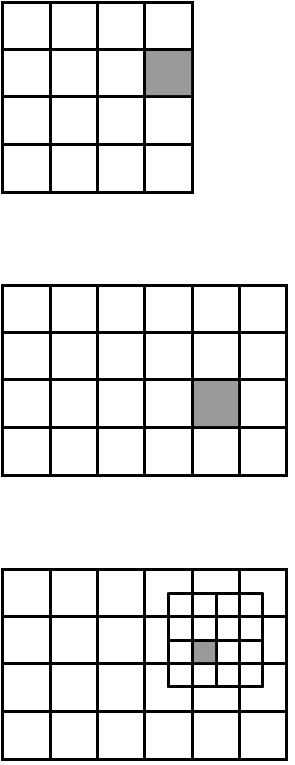
\includegraphics[scale=0.4]{figs/gridsearch.jpg}
	\end{center}
	\caption{Diagrams illustrating how the hyperparameter search is conducted.}
	\label{fig:gridsearch}
\end{figure}

\subsubsection{Dimensionality Reduction} \label{impl-reduction}

The running time of an SVM classifier increases with the size of the features. It therefore makes sense to use dimensionality reduction techniques to improve the efficiency of classification. In this project, I used principle component analysis (PCA), as it is a relatively efficient method and there is good library support for it. Initially, I used the Scikit-learn implementation of PCA \cite{sklearnpca}, however after testing it I found that I could perform the feature reduction more efficiently using the NumPy singular value decomposition function \cite{numpysvd} and using the resulting matrices to perform reduce the size of the features (which is how PCA is carried out \cite{svd}). Listing \ref{lst:reduce_features} gives my Python code for this dimensionality reduction. As discussed in \ref{eval-reduction}, even the NumPy implementation was too slow to be practical in the project and good results could by reducing the size of the features by limiting the number of words considered.

\pylisting{A function using NumPy array operations to perform singular value decomposition on two sets of given features}{reduce_features}

\section{Summary}

In this chapter I described the overall system architecture and discussed the work I undertook to implement the project's components. Throughout the preparation and implementation, I made decisions to facilitate the evaluation, which is detailed further in the next chapter.

\chapter{Evaluation} \label{eval}

In this section I assess the successes and failures of what was developed in this project. To follow a similar order to the implementation section, I first analyse the data in section \S\ref{eval-database}, then evaluate the classifier's results in section \S\ref{eval-results} and in section \S\ref{eval-reduction} I consider the benefits of the extension in which I implemented dimensionality reduction. I then move onto section \S\ref{eval-spam} in which I evaluate my results for the spam email classifier. I conclude this chapter by assessing the extent to which the project met its goals in section \S\ref{eval-goals}.

\section{Database Analysis} \label{eval-database}

Since the result of the data acquisition described in section \S\ref{impl-acquisition} was a dataset of predominantly textual, it was difficult to quantitatively analyse this part of the project, but I performed various checks in order to establish that the dataset was constructed correctly.
\\\\
Firstly, the defensive programming style I adopted when writing the code to fetch, collate and store the data was geared towards facilitating the evaluation - wherever there was an error with the data, I outputted the relevant information and didn't write the data to the database. I then manually checked these outputs to see if there were any data that should have been written to the database, but wasn't due to the error. All of the outputs related to instances where there were problems with the Hansard, which indicates that my program to create the database worked correctly.
\\\\
Another way I assessed the database was to perform a series of unit tests on the database class's methods. For these tests, I used the original data sources (the Hansard and data.parliament.uk) to create a series of expected outputs from a set of queries I wrote. I then ran the queries and the actual results were 100\% consistent with the expected results. Further to this, when accessing the data to develop the project's classifier, the database never produced an error. Given that the primary function of the database was to be used for this classifier, this supports success of the database acquisition section of the project.
\\\\
The main quantitative analysis I carried out on the database was considering the word (and n-gram) frequency distribution. According to Zipf's law, the frequency of the $i^{th}$ most frequent term is inversely proportional to $i$ (the word's rank). More specifically, there is a linear relationship between the logarithm of the frequency of a word and the logarithm of the rank of the word \cite{zipf}. Although Zipf's law is just an empirical observation, if the database was constructed correctly, we would expect it to obey this rule. Figure \ref{fig:bigzipf} shows a scatter plot of frequency against rank for all the words in the debates considered in this project, constructed using the project's database. The graph is plotted on a log-log scale, which is why we see the linear correlation that we would expect of a natural corpus. The coefficient of determination, $r^2$, for the plotted data is $0.97 \pm 0.07$\footnote{Although the standard error suggests it could be, the coefficient of determination cannot exceed 1.}, which provides further evidence for the project's corpus obeying Zipf's law and supports my hypothesis that it is properly constructed. 
\\\\
\begin{figure}
	\begin{center}
		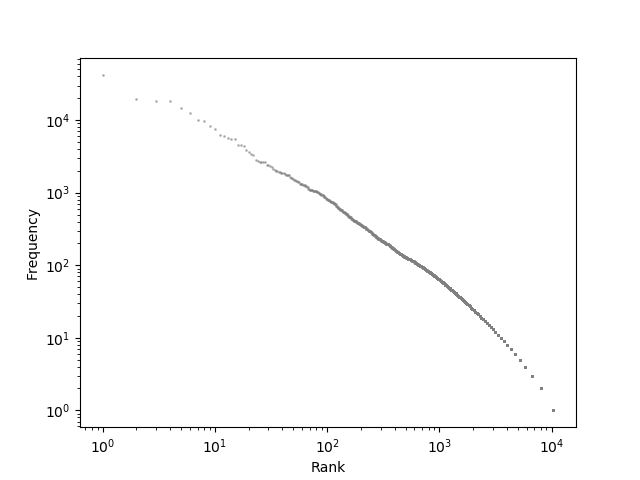
\includegraphics[scale=1]{figs/bigzipf.png}
	\end{center}
	\caption{A scatter plot of frequency against rank for all the words in the debates considered in this project.}
	\label{fig:bigzipf}
\end{figure}

Figure \ref{fig:ngramoffset} is another scatter plot of the same 500 terms, but instead plots their probability offset against their frequency (on a log scale). The probability offset of a given term is given by:
\begin{equation}
	\frac{\sum_{s \in P}c_{s}(\text{term})}{\sum_{s \in P \cup N}c_{s}(\text{term})} - \frac{\sum_{t \in T}\sum_{s \in P}c_{s}(t)}{\sum_{t \in T}\sum_{s \in P \cup N}c_{s}(t)}
\end{equation}
where $c_{s}(t)$ is the occurrences of term $t$ in speech $s$, $T$ is the set of the 500 most common words and 2-grams in the training set, $P$ is the set of positively labelled (pro-war) speeches in the training set and $N$ is the set of negatively labelled (anti-war) speeches in the training set. The first part of the expression corresponds to the probability of an occurrence of the given term being in a pro-war speech, while the second part is the probability that a given occurrence of any term is in a pro-war speech. This normalisation is necessary due to the fact that the dataset is unbalanced. Any terms for which the probability offset is greater than 0 have a pro-war bias and any term with a probability offset less than 0 have an anti-war bias. The figure shows that the more common terms do not have significant biases, but less frequent terms are more likely to be useful to our classification. Table \ref{table:anti-grams} and table \ref{table:pro-grams} show the most anti-war and pro-war terms respectively, while table \ref{table:databasestats} gives other statistics about the contents of the database.
\\\\
\begin{figure}
	\begin{center}
		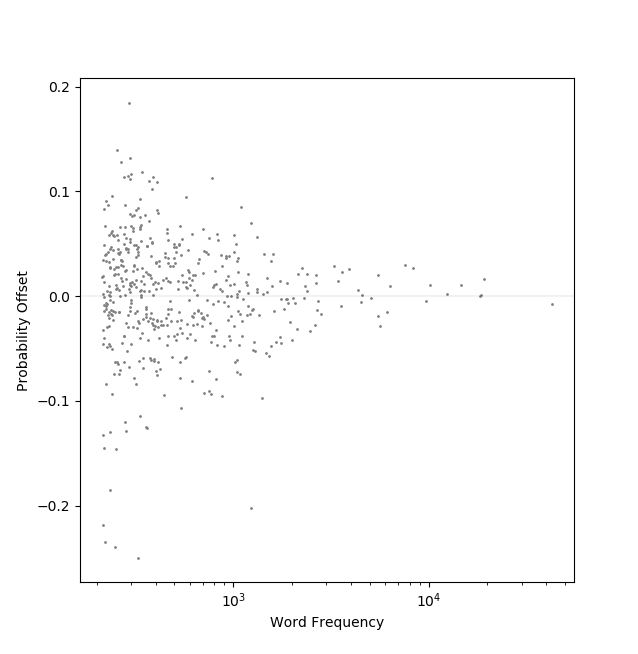
\includegraphics[scale=0.8]{figs/ngramoffset.png}
	\end{center}
	\caption{A scatter plot of probability offset against frequency for the 500 most common words and 2-grams in the training set.}
	\label{fig:ngramoffset}
\end{figure} 

\begin{table}[]
	\centering
	\begin{tabular}{lll}
		\hline
		\textbf{Term}  & \textbf{Probability Offset} & \textbf{Frequency} \\ \hline
		war iraq&-0.621&64\\
		cluster bomb&-0.484&69\\
		cluster&-0.442&73\\
		british govern&-0.409&56\\
		oil&-0.3219&93\\
		go war&-0.291&82\\
		billion&-0.290&50\\
		mani us&-0.270&50\\
		bomb&-0.249&432\\
		georg&-0.249&81\\
		nuclear weapon&-0.246&95\\
		bush&-0.242&250\\
		drop&-0.237&67\\
		court&-0.230&104\\
		conserv&-0.230&98\\
		american&-0.219&444\\
		tell us&-0.216&74\\
		authoris&-0.215&68\\
		administr&-0.212&228\\
		fire&-0.211&77\\ \hline
	\end{tabular}
	\caption{The 20 most anti-war n-grams that occur at least 50 times in the debates considered in this project.}
	\label{table:anti-grams}
\end{table}
\begin{table}[]
	\centering
	\begin{tabular}{lll}
		\hline
		\textbf{Term} & \textbf{Probability Offset} & \textbf{Frequency} \\ \hline
		grate hon&0.233652194&55\\
		royal marin&0.229475289&74\\
		river&0.220996222&102\\
		interim&0.212323522&52\\
		chapter&0.209409769&66\\
		state israel&0.203349163&60\\
		brigad&0.201050313&58\\
		complianc&0.200571386&72\\
		board&0.199840391&57\\
		regiment&0.195941756&54\\
		novemb&0.194258254&66\\
		avail&0.190650751&189\\
		taliban regim&0.186682497&72\\
		saddam',0.182103742&91\\
		practic&0.181780536&68\\
		emphasis&0.180730116&56\\
		palestinian author&0.177232325&97\\
		reconstruct&0.175898183&85\\
		educ&0.175676207&53\\
		deliv&0.173524602&114\\ \hline
	\end{tabular}
	\caption{The 20 most pro-war n-grams that occur at least 50 times in the debates considered in this project.}
	\label{table:pro-grams}	
\end{table}
\begin{table}[]
	\centering
	\begin{tabular}{lll}
		\hline
		\textbf{Quantity} & \textbf{Total} & \textbf{Used by Classifier} \\ \hline
		MPs               & 655            & 276                         \\
		Speeches          & 19,513         & 2,83                        \\
		Debates           & 1578           & 36                          \\ 
		Tokens            & 4,189,328      & 592,295                     \\
		Distinct words    & 57,288         & 19,254                      \\ \hline
	\end{tabular}
	\caption{A breakdown of the numbers in the database.}
	\label{table:databasestats}	
\end{table}
\section{Classifier Results} \label{eval-results}

Table \ref{table:results} highlights the successful performance of the classifier I developed for this project - it significantly outperforms the na\"{i}ve Bayes classifier, which I decided would be the baseline in the initial stages of the project. Note that I have used F1 scores as the metric to compare classifiers, as F1 scores account for imbalances in data, as I discussed in section \S\ref{evaluation-metrics}.
\\\\
\begin{table}[]
	\centering
	\begin{tabular}{lll}
		\hline
		\textbf{Classifier}      & \textbf{F1 score by speech} & \textbf{F1 score by MP} \\ \hline
		Na\"{i}ve Bayes baseline & 0.392                       & 0.182                   \\
		SVM                      & 0.894                       & 0.809                   \\ \hline
	\end{tabular}
	\caption{The F1 scores of the project's main classifier and the baseline classifier.}
	\label{table:results}	
\end{table}

The cross-validation learning algorithm established that the rbf kernel function would likely produce the best results. In doing so, it performed a search for the best combination of hyperparameters (as described in section \S\ref{impl-learning}). Figure \ref{fig:hyperparamgrid} illustrates the first iteration of the grid search for hyperparameters. The diagram clearly shows that lower values of $C$ result in a better F1 score. This is expected, as lower values of $C$ allow more training examples to be misclassified (as discussed in section \S\ref{prep-svm}) and there is inherent noise in the data, due to MPs not voting consistently with their own views due to party whips \cite{whips}, which results in some mislabelling of the data.
\\\\

\begin{figure}
	\begin{center}
		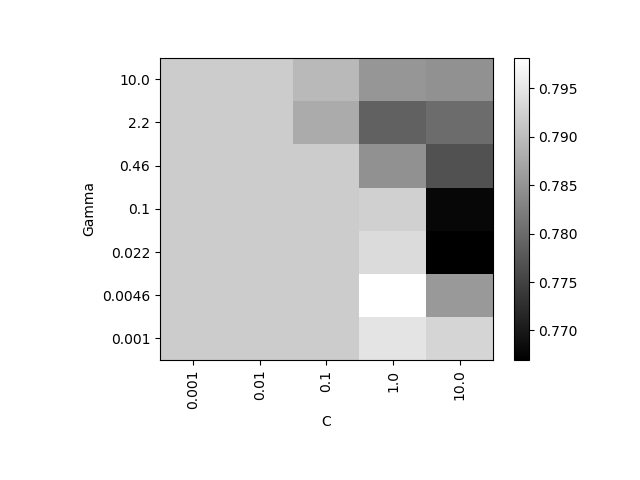
\includegraphics[scale=0.8]{figs/hyperparamgrid.png}
	\end{center}
	\caption{A diagram showing the grid of the first stage of the hyperparameter search.}
	\label{fig:hyperparamgrid}
\end{figure}

The learning algorithm which determined the kernel and hyperparameters also determined the settings, which are shown in table \ref{table:settings}. As tables \ref{table:anti-grams} and \ref{table:pro-grams} demonstrate, 2-grams were very useful in classification, so it makes sense that the learning algorithm chose to use them. The tables also show that stop words do carry significant semantic value when they are part of a 2-gram, despite the fact that figure \ref{fig:ngramoffset} shows that stop words are not useful in isolation for classification. Although it may be useful to group numbers for some applications, it was not in this case, as evidenced by the fact that `September 11' had a significant anti-war bias and `1441' was the 15th most pro-war term (the United Nations Security Council Resolution 1441 was an offering to Iraq to encourage them to disarm \cite{resolution}).
\\\\
Interestingly, table \ref{table:results} shows that for both classifiers, the F1 score was higher when was calculated on predictions for each speech, rather than on predictions for each MP. This is counter-intuitive, since the MPs' predictions are made using an aggregation of their speeches - we might expect that having more data would lead to better classifications. The most feasible explanation is that speeches made by MPs who make less speeches are more likely to be misclassified. This makes sense, since if an MP is less sure of their stance on the war, their view is more likely to have changed over the period of time from which this project's corpus was created. Further to this, an MP who is less sure of their stance is more likely to be convinced to follow their party's line. I decided to test the hypothesis that MPs who made less speeches in debates related to the Iraq war were more likely to be misclassified, by carrying out a t-test. The mean of the number of speeches made for correctly classified MPs was 10, whereas it was only 5 for misclassified MPs. While this does support the hypothesis, the t statistic was 0.951, meaning it was only significant to the 80\% level, which is not sufficiently high to make any conclusive statements about the hypothesis.

\begin{table}[]
	\centering
	\begin{tabular}{ll}
		\hline
		\textbf{Setting}  & \textbf{Value} \\ \hline
		n\_gram           & 5              \\ 
		remove\_stopwords & True           \\
		stem\_words       & True           \\
		group\_numbers    & False          \\
		normalise         & True           \\
		\hline
	\end{tabular}
	\caption{The settings learned by the SVM classifier.}
	\label{table:settings}	
\end{table}

\section{Evaluation of Dimensionality Reduction} \label{eval-reduction}

When testing the principle component analysis (PCA) I had implemented (see section \S\ref{impl-reduction}), I realised that the slow operation of the singular value decomposition (svd - part of the principle component analysis algorithm) had become the bottleneck on the running time of the classifier and the gains in performance it achieved were marginal. The poor running time was due to the fact that the feature vectors that the algorithm was decomposing were so large. I therefore decided to truncate these vectors by decreasing the bag size in the bag of words model, before performing the svd. While this did significantly speed-up the PCA, it resulted in a lower F1 score than could be achieved by truncating the feature vectors to the same dimensionality, just by decreasing bag size. Since decreasing the bag size had no time overhead and produced better results, I decided to use this in the classifier and omit the use of PCA entirely.


\section{Spam Email Dataset} \label{eval-spam}

As discussed in section \S\ref{impl-overfitting}, developing a classifier to detect spam email before the project's main classifier had many benefits, including adding a further way to evaluate the system. This evaluation is possible, since the spam email dataset I used was published by Medlock along with a paper containing state-of-the-art results for spam email detection \cite{spampaper}, meaning that I could compare these results with my own. My classifier achieved 90\% accuracy\footnote{I give the accuracy rather than F1 score here, since this is what is used in the paper which I am using to compare my results.} on the spam email dataset, compared with the 93\% given in Medlock's paper for SVM classification. Since this classifier was specifically tailored to detecting spam email and mine was not (since spam detection was not the focus of this project), the 90\% accuracy my classifier achieved is a respectable result.

\section{Evaluation of Project Goals} \label{eval-goals}

The two primary goals of the project were defined in section \S\ref{prep-requirements}. They were to ``Construct a database that comprises British texts on the Iraq war'' and to ``Develop a classifier that can determine the stance of the texts in the database''. Section \S\ref{eval-database} provides evidence of my achievement of the first of these goals and section \S\ref{eval-results} shows that I have successfully completed the second of the two goals. I refined these goals to give the project's core tasks in table \ref{table:tasks}, which I completed (as detailed in \S\ref{impl}), before going on to complete extensions to the project.

\section{Summary}

This project was successful in achieving two main aims of creating a dataset of British texts on the Iraq war and developing a classifier to use this corpus. The novel method of using an MPs' House of Commons voting record to label their speeches proved to be successful, as demonstrated by the good results of the classifier.

\chapter{Conclusions} \label{conc}

\section{Achievements}

Through carrying out this project, I created a dataset using data from the Hansard and data.parliament.uk. This dataset contains all the speeches and votes made between September 11th 2001 and 18th March 2003 (inclusive). I then used this dataset to develop an SVM classifier which achieved an F1 score of 0.898 on MPs' speeches, which is significantly better than the baseline 0.392, which was the F1 score of the na\"{i}ve Bayes classifier on the same data.

\section{Lessons Learned}

The success of the project demonstrates that the Hansard is a great resource for NLP applications, especially as I showed that it can be labelled using House of Commons voting data. While the project did go well overall, the licensing issues with the initial dataset delayed the project from the off. If I were to do the project again, I would check the licences of the any resources it was using before starting any other work, so as to avoid a similar problem. In addition to learning more about licensing of data, I learned a lot about NLP and machine learning techniques through carrying out this project.

\section{Future Work}

To improve the classifier, I could adopt more complex models which could account for how MPs' stances change over time or how likely an MP is to follow their party's line in a vote when they contradict the MPs own views. A new model could also use additional data from other sources, such as newspapers and social media to further improve classification. The dataset could be extended over a longer range, thus making it useful for analyses of a wider range of political issues. I plan to create an API for this dataset, which will hopefully encourage further applications to be built using House of Commons data, which would in turn increase the accountability of MPs.

\begin{comment}
This chapter is likely to be very short and it may well refer back to the Introduction. It might properly explain how you would have planned the project if starting again with the benefit of hindsight.
\end{comment}


%%%%%%%%%%%%%%%%%%%%%%%%%%%%%%%%%%%%%%%%%%%%%%%%%%%%%%%%%%%%%%%%%%%%%
% the bibliography
\addcontentsline{toc}{chapter}{Bibliography}
\bibliography{refs}

%%%%%%%%%%%%%%%%%%%%%%%%%%%%%%%%%%%%%%%%%%%%%%%%%%%%%%%%%%%%%%%%%%%%%
% the appendices
\appendix

\chapter{Project Proposal}
\label{sec:proposal}
\documentclass[12pt,a4paper,twoside]{article}
\usepackage[pdfborder={0 0 0}]{hyperref}
\usepackage[margin=25mm]{geometry}
\usepackage{graphicx}
\usepackage{parskip}
\begin{document}

\begin{center}
\Large
Computer Science Tripos -- Part II -- Project Proposal\\[4mm]
\LARGE
Sentiment Analysis of British Newspaper Articles on the Iraq War

\large
Louis Slater, Pembroke College

Originator: Louis Slater

12th October 2017
\end{center}

\vspace{5mm}

\textbf{Project Supervisor:} Dr Tamara Polajnar

\textbf{Director of Studies:} Dr Anil Madhavapeddy

\textbf{Project Overseers:} Dr Timothy Griffin \& Professor Anuj Dawar

% Main document

\section*{Introduction}
While there have been lots of studies involving sentiment analysis of political texts to determine their bias, none of these have uniquely involved British newspaper articles. Furthermore, after extensive research, I have not found any sentiment analysis of articles to determine their stance on a war. The purpose of this project is to develop a program that can reasonably determine the stance of any British newspaper article on the Iraq war. The core part of this project will be developing a program that achieves this using a bag-of-words method.

\section*{Starting point}
In the past few years, there has been a lot of research into determining political biases of shorter segments of text, such as Tweets in the 2010 paper by Pak and Paroubek on ‘Twitter as a Corpus for Sentiment Analysis and Opinion Mining’. On the other hand, ‘Political Ideology Detection Using Recursive Neural Networks’ by Iyyer, Enns, Boyd-Graber and Resnik uses a corpus containing longer texts – US Congressional floor debate transcripts. Although there are clear differences between these transcripts and the newspaper articles that I plan to use (for example, the fact that the transcripts were initially spoken, whereas the articles were not), there are also many similarities (for example the length and inherently political nature of the corpora). Since this study showed that a bag-of-words method can successfully determine the bias of these transcripts with a 65\% accuracy, it is justified to use a similar model to determine the bias of the newspaper articles I shall analyse.

The corpus I will use will be articles on the Iraq war from up to seven of the UK’s most popular national daily newspapers and their Sunday equivalents published between 16th March 2003 and 18th April 2003. I will use a database of these articles compiled by Robinson, Goddard, Brown and Taylor in their 2003 study, ‘Content and Framing Study of United Kingdom Media Coverage of the Iraq War’, in which they manually determine the stance of 4,893 news articles from seven British daily newspapers and their Sunday equivalents (Daily Telegraph, The Times, The Guardian/The Observer, The Independent, The Daily Mail, The Mirror, The Sun/News of the World). This database does not include the articles’ texts, so the first part of my implementation will be to scrape this data from as many of these articles as possible. I will be able to get these texts from existing online Newspaper archives. I have already found searchable archives for The Guardian, The Observer, The Daily Telegraph, The Sunday Telegraph, The Independent, Indy on Sunday, The Times and the Sunday Times, all of which I will be able to use. Scraping textual data from the other newspapers in the database may be prove more difficult, but I will as many possibilities as I feasibly can within the scope of the project.

\section*{Resources required}
In addition to the database and archives mentioned above, I will also require the use of a computer. I intend to mainly use my own computer, which has an Intel Core i7 processor and runs Windows 10. I will use the computing facilities in my college if my laptop is lost, broken or stolen. I will back up my work using both Google Drive and GitHub, which I will also use as a version control repository. I may also require the use of a server or external hard drive to store the corpus I use; however, this will be dependent on the amount of data that I scrape in the initial part of my project.

\section*{Work to be done}
The project breaks down into the following sub-projects:

\begin{enumerate}

\item Gaining access to as many of the relevant searchable newspaper archives as possible.
\item Scraping data from as many articles as possible in the database compiled by Robinson, Goddard, Brown and Taylor.
\item Implementing a program to determine the biases of texts on the Iraq war, using the corpus I gather, along with corresponding the Reporter’s Tones from the database compiled by Robinson, Goddard, Brown and Taylor.
\item Running the program on the texts and comparing the results with the manually determined biases to judge the effectiveness of the program.

\end{enumerate}

\section*{Success citeria}
The project will be a success if I develop a program that can determine the stance of an article on the Iraq war with a greater than 50\% accuracy.

\section*{Possible extensions}
If I meet my success criteria early, I shall attempt one, or both, of the following extensions:

\begin{itemize}

\item Implementing a program that performs the same function as the initial program I develop, but using a different method, such as a recursive neural network. If I complete this extension, I will be able to compare the effectiveness of the two methods.
\item Extrapolating the results using new datasets and analysing these results. Possible datasets I could use are newspaper articles from different countries, publications or times or transcripts of parliamentary debates.

\end{itemize}



\section*{Timetable}

Planned starting date is the beginning of Michaelmas Week 3 (Thursday 19th October 2017).

\begin{enumerate}

\item \textbf{Michaelmas week 3} Gain access to as many of the relevant searchable newspaper archives as possible.

\item \textbf{Michaelmas weeks 4--5} Scrape data from as many articles as possible in the database compiled by Robinson, Goddard, Brown and Taylor, creating a database of the texts, their manually determined bias and other relevant information on them. If necessary, I will also get access to a server and store the database I compile on this server.

\item \textbf{Michaelmas weeks 6--8} Implement a program to determine the biases of texts on the Iraq war, using the corpus I gather, along with corresponding the Reporter’s Tones from the database compiled by Robinson, Goddard, Brown and Taylor.

\item \textbf{Michaelmas vacation} Finish the implementation, then run the program on the texts and compare the results with the manually determined biases to judge the effectiveness of the program.

\item \textbf{Lent weeks 1--2} Write the progress report and start work on possible extensions of the project.

\item \textbf{Lent weeks 3--4} Finish the extensions to the project.

\item \textbf{Lent weeks 5--6} Write the first draft of the dissertation.

\item \textbf{Lent weeks 7--8} Revise the dissertation in accordance with feedback I receive from my supervisor.

\item \textbf{Easter vacation} Finish revising the dissertation and submit the final project.

\end{enumerate}

\end{document}


\end{document}
